% Intended LaTeX compiler: pdflatex


\documentclass[12pt]{article}
% \usepackage[includeheadfoot,margin=1.0in,hmargin=1.0in,vmargin=0.5in]{geometry} % for normal margins
\usepackage[includeheadfoot,margin=1.5in,hmargin=1.5in,vmargin=0.5in]{geometry} % for insanely wide margins
% \usepackage[includeheadfoot,margin=2.0in,hmargin=2.0in,vmargin=0.5in]{geometry} % for insanely wide margins
\usepackage{float}


\usepackage{algorithm}
\usepackage{amsmath}
\usepackage{ifxetex}
\ifxetex
  \usepackage{fontspec,xltxtra,xunicode}
  \defaultfontfeatures{Mapping=tex-text,Scale=MatchLowercase}
  \setromanfont{Garamond Premier Pro}
%  \setromanfont{Adobe Caslon Pro}
 \setsansfont{Gotham Narrow Bold}
  \setmonofont{Myriad Pro}
\else
  \usepackage[mathletters]{ucs}
  \usepackage[utf8x]{inputenc}
\fi
\usepackage{url}
\usepackage{paralist}
\usepackage{graphicx}
\usepackage{tikz}
\usepackage{calc}
\usepackage{eso-pic}
\usepackage{etoolbox}
\usepackage{xcolor}
\PassOptionsToPackage{hyperref,x11names}{xcolor}
\definecolor{pinterestred}{HTML}{C92228}
\definecolor{ulyssesbutterflyblue}{HTML}{1464F4}
\definecolor{signalflare}{HTML}{FB782C}
\definecolor{niceorange}{HTML}{77CC6D}
\definecolor{highlighteryellow}{HTML}{FFFF01}
\definecolor{ghostlygrey}{HTML}{000000}
\definecolor{firstcolor}{HTML}{00ADEF}
\definecolor{secondcolor}{HTML}{DD3E74}
\definecolor{periodblue}{HTML}{12239e}
\definecolor{denimblue}{HTML}{3A5F90}
\definecolor{electricblue}{HTML}{05ADF3}


\newtoks\leftheader 
\newtoks\leftheaderurl
\newtoks\coverimage


\hyphenpenalty=5000 
\tolerance=1000

%This macro is to make cleaner the specification of the titling font
\newfontfamily\mytitlefont[Color={highlighteryellow}]{Gotham Narrow Bold}
\newfontfamily\myauthorfont[Color={highlighteryellow}]{Gotham Narrow Bold}
\newfontfamily\mybluefont[Color=electricblue]{Gotham Narrow Bold}
\DeclareTextFontCommand{\textbf}{\bfseries\color{electricblue}}
\DeclareTextFontCommand{\textit}{\itshape}


\usepackage{textcase}

\pagenumbering{arabic}
\makeatletter

%This macro now controls the position of the background pic
%Please do not change from here
\newcommand\BackgroundPic{%
\put(0,0){%
\parbox[b][\paperheight]{\paperwidth}{%
\vfill
\centering
%inside the tikzpicture environment, you can do anything you want with the image
\begin{tikzpicture}

\node [inner sep=0pt,outer sep=0pt] at (0,0) {\includegraphics[width=\paperwidth,height=\paperheight]{\the\coverimage}};

\node at  (0,5) [opacity=1.0] {\parbox[b][0.5\textheight]{\textwidth}{%
  \begin{raggedright}
  \leavevmode
    \vskip 1cm
  {\mytitlefont\fontsize{75}{85}\bfseries{\@title}\par}
    \vskip 1cm
    
    %{\myauthorfont\fontsize{30}{40}{{\bfseries{\@degree}\par}}}

\vfill
\end{raggedright}}};
\node at (0,-8) [opacity=1] {\parbox[b][0.3\textheight]{\textwidth}{%
\begin{raggedright}
\vfill
{\myauthorfont\Large {\@author}}
    \newline
          {\myauthorfont\Large \href{mailto:jay@storytelling.nyc}{jay@storytelling.nyc}}
        \newline
{\myauthorfont\Large
\href{http://storytelling.nyc}{Storytelling.NYC}}
\newline
{\myauthorfont\Large © 2017 \@author}
    \newline
%{\myauthorfont\Large Private and Confidential}
 %   \newline
        \newline
    {\myauthorfont\Large \@date\par}
%{\myauthorfont\Large \href{http://jaydixit.com}{\@degree }}
\end{raggedright}
}};
\end{tikzpicture}
%Don't change
\vfill
}}}
%This macro executes a hook at the beginning of the document that  puts the background correctly. 
\AtBeginDocument{\AddToShipoutPicture*{\BackgroundPic}}
\AtBeginDocument{\globalcolor{ghostlygrey}}



%The maketitle macro now only includes the titling and not the background. 
\def\maketitle{ \newgeometry{margin=1in} \thispagestyle{empty} \vfill \null \cleardoublepage\restoregeometry}



\setcounter{secnumdepth}{0}




\usepackage{fancyhdr}
\pagestyle{fancy}
\renewcommand{\sectionmark}[1]{\markboth{#1}{}}
\lhead{\href{\the\leftheaderurl}{\the\leftheader}}
\chead{}
\rhead{\@title: {\nouppercase{\leftmark}}}
\lfoot{}
\cfoot{}
\rfoot{}
\usepackage{listings}
\setlength{\parindent}{0pt}
\setlength{\parskip}{12pt plus 2pt minus 1pt} %Space between paragraphs
\usepackage{fancyvrb}
\usepackage{enumerate}
\usepackage{ctable}
\setlength{\paperwidth}{8.5in}
\setlength{\paperheight}{11in}
  \tolerance=1000
\usepackage{tocloft}
\renewcommand{\cftsecleader}{\cftdotfill{\cftdotsep}}
\usepackage[normalem]{ulem}


\makeatletter
\newcommand{\globalcolor}[1]{%
  \color{#1}\global\let\default@color\current@color
}
\makeatother

\newcommand{\textsubscr}[1]{\ensuremath{_{\scriptsize\textrm{#1}}}}

\usepackage{enumitem}
\newlist{mylist}{enumerate}{10} 
%\setlist{nolistsep}
\setlist{topsep=0pt}
\renewcommand{\labelitemi}{\raise 0.25ex\hbox{\tiny$\bullet$}}
\renewcommand{\labelitemii}{\raise 0.25ex\hbox{\tiny$\bullet$}}
\renewcommand{\labelitemiii}{\raise 0.25ex\hbox{\tiny$\bullet$}}
\renewcommand{\labelitemiv}{\raise 0.25ex\hbox{\tiny$\bullet$}}
\renewcommand{\labelitemv}{\raise 0.25ex\hbox{\tiny$\bullet$}}
\renewcommand{\labelitemvi}{\raise 0.25ex\hbox{\tiny$\bullet$}}
\renewcommand{\labelitemvii}{\raise 0.25ex\hbox{\tiny$\bullet$}}
\renewcommand{\labelitemviii}{\raise 0.25ex\hbox{\tiny$\bullet$}}
\renewcommand{\labelitemix}{\raise 0.25ex\hbox{\tiny$\bullet$}}
\renewcommand{\labelitemx}{\raise 0.25ex\hbox{\tiny$\bullet$}}

\setlistdepth{10}
\setlist[itemize,1]{label=\raise 0.25ex\hbox\tiny$\bullet$}
\setlist[itemize,2]{label=\raise 0.25ex\hbox\tiny$\bullet$}
\setlist[itemize,3]{label=\raise 0.25ex\hbox\tiny$\bullet$}
\setlist[itemize,4]{label=\raise 0.25ex\hbox\tiny$\bullet$}
\setlist[itemize,5]{label=\raise 0.25ex\hbox\tiny$\bullet$}
\setlist[itemize,6]{label=\raise 0.25ex\hbox\tiny$\bullet$}
\setlist[itemize,7]{label=\raise 0.25ex\hbox\tiny$\bullet$}
\setlist[itemize,8]{label=\raise 0.25ex\hbox\tiny$\bullet$}
\setlist[itemize,9]{label=\raise 0.25ex\hbox\tiny$\bullet$}
\setlist[itemize,10]{label=\raise 0.25ex\hbox\tiny$\bullet$}
\renewlist{itemize}{itemize}{10}





\definecolor{azure}{HTML}{f2feff}

\usepackage{lipsum}
\usepackage{tikz}
\usetikzlibrary{backgrounds}
\makeatletter

\tikzset{%
  fancy quotes/.style={
    text width=\fq@width pt,
    align=justify,
    inner sep=1em,
    anchor=north west,
    minimum width=\linewidth,
  },
  fancy quotes width/.initial={.8\linewidth},
  fancy quotes marks/.style={
    scale=8,
    text=black,
    inner sep=0pt,
  },
  fancy quotes opening/.style={
    fancy quotes marks,
  },
  fancy quotes closing/.style={
    fancy quotes marks,
  },
  fancy quotes background/.style={
    show background rectangle,
    inner frame xsep=0pt,
    background rectangle/.style={
      fill=azure,
      rounded corners,
    },
  }
}

\newenvironment{fancyquotes}[1][]{%
\noindent
\tikzpicture[fancy quotes background]
\node[fancy quotes opening,anchor=north west] (fq@ul) at (0,0) {``};
\tikz@scan@one@point\pgfutil@firstofone(fq@ul.east)
\pgfmathsetmacro{\fq@width}{\linewidth - 2*\pgf@x}
\node[fancy quotes,#1] (fq@txt) at (fq@ul.north west) \bgroup}
{\egroup;
\node[overlay,fancy quotes closing,anchor=east] at (fq@txt.south east) {''};
\endtikzpicture}
\makeatother


\usepackage{setspace}
\usepackage{lipsum}
\usepackage{etoolbox}
\AtBeginEnvironment{quote}{\singlespace\vspace{-\topsep}\small}
\AtEndEnvironment{quote}{\vspace{-\topsep}\endsinglespace}


\usepackage[sc]{titlesec}
\titlespacing*{\section}{0pt}{6pt}{7pt}
\titlespacing*{\subsection}{0pt}{0pt}{7pt}
\titlespacing*{\subsubsection}{0pt}{6pt}{5pt}

\titleformat*{\section}{\normalfont\fontsize{36}{36}\raggedright\bfseries\sffamily\color{pinterestred}}
\titleformat*{\subsection}{\normalfont\fontsize{20}{20}\scshape\color{electricblue}}
\titleformat*{\subsubsection}{\normalfont\fontsize{12}{8}\raggedright\bfseries\rmfamily\color{pinterestred}}
\titleformat*{\paragraph}{\normalfont\normalsize\raggedright\bfseries\rmfamily\color{electricblue}}
\titleformat*{\subparagraph}{\normalfont\fontsize{14}{14}\raggedright\bfseries\ttfamily\color{pinterestred}}
\usepackage[breaklinks=true,linktocpage,xetex]{hyperref} 
\hypersetup{colorlinks, citecolor=electricblue,filecolor=electricblue,linkcolor=electricblue,urlcolor=electricblue}




      

\setcounter{secnumdepth}{0}
\setcounter{tocdepth}{3}
\leftheader{Jay Dixit}
\leftheaderurl{http://jaydixit.com}
\coverimage{/Users/jay/emacs/emacs-settings/new-latex-templates/images/image1.jpg}
\author{Jay Dixit Jay Dixit}
\date{\today}
\title{Effective Emails Alice in Wonderland}
\hypersetup{
 pdfauthor={Jay Dixit Jay Dixit},
 pdftitle={Effective Emails Alice in Wonderland},
 pdfkeywords={},
 pdfsubject={},
 pdfcreator={Emacs 25.1.1 (Org mode 9.1.2)}, 
 pdflang={English}}
\begin{document}

\maketitle
\tableofcontents
\newpage





\section{curiosity}
\label{sec:org30d1650}
\begin{quote}
Humans have a natural desire for closure– we don’t like having gaps in our knowledge. You can leverage this desire for closure by leaving your subject line open-ended so subscribers will be curious, like a cliffhanger that can only be satisfied by opening the email. You can make subscribers curious by asking a question (and answering it in your email), promising something interesting (like pictures or a surprise gift), or simply saying something that sounds strange or unusual.
\end{quote}
\textbf{Source:} \href{///Users/jay/devonthink-databases/NLI.dtBase2/Files.noindex/pdf/b/Revealed-\%20164\%20Best\%20Email\%20Subject\%20Lines\%20to\%20Boost\%20Open\%20Rates\%20(Updated).pdf::1}{Revealed- 164 Best Email Subject Lines to Boost Open Rates (Updated).pdf, p. 1}




\section{Intro}
\label{sec:orgccb5a32}


\subsection[Effective Emails]{Effective Emails\hfill{}\textsc{slide:aligncenter}}
\label{sec:org5ff203c}

\textbf{Jay Dixit} \\
Storytelling.NYC \\
jay@storytelling.nyc \\

\begin{center}

\includegraphics[width=.9\linewidth]{/Users/jay/Dropbox/github/org-html-webslides/assets/img/storytelling-nyc-logo-new-face.png}
\end{center}

\subsubsection[Notes]{Notes\hfill{}\textsc{notes}}
\label{sec:orgdaf34bc}
Welcome everyone. My name is Jay Dixit.

\subsection[Effective Emails]{Effective Emails\hfill{}\textsc{slide:aligncenter}}
\label{sec:org90d080d}
\subsubsection[Notes]{Notes\hfill{}\textsc{notes}}
\label{sec:org415fb1b}
Today we're going to talk about how to write effective emails.

\subsection[Effective \textit{Sales} Emails]{Effective \textit{Sales} Emails\hfill{}\textsc{slide:aligncenter}}
\label{sec:orga55741a}

\subsubsection[Notes]{Notes\hfill{}\textsc{notes}}
\label{sec:org6b393ff}
Specifically, effective \textbf{sales} emails.
\subsection[Effective Sales \textit{Response} Emails]{Effective Sales \textit{Response} Emails\hfill{}\textsc{slide:aligncenter}}
\label{sec:org11e9202}

\subsubsection[Notes]{Notes\hfill{}\textsc{notes}}
\label{sec:orgf50fed0}
And specifically, \textbf{today} we're going to talk about how to get better at writing \textbf{response} emails to prospects.

Sooooooo. I want going to start by asking you guys a question.

\subsection[What do typically think about when we write emails?]{What do typically think about when we write emails?\hfill{}\textsc{slide}}
\label{sec:orge1f1056}

\subsubsection[Notes]{Notes\hfill{}\textsc{notes}}
\label{sec:org99afe25}
What \textbf{questions} do you usually ask yourself as you're writing an email?
\begin{itemize}
\item what should I say?
\item what information should I include?
\item what links
\item where do I draw information from
\end{itemize}

These are \textbf{low-level of construal.}

I want to give you guys a framework for thinking about this in a different way.

So we can develop \textbf{habits}.

\subsection[Pop goes the]{Pop goes the\hfill{}\textsc{slide:full:invisible}}
\label{sec:org2f544e3}
\begin{center}
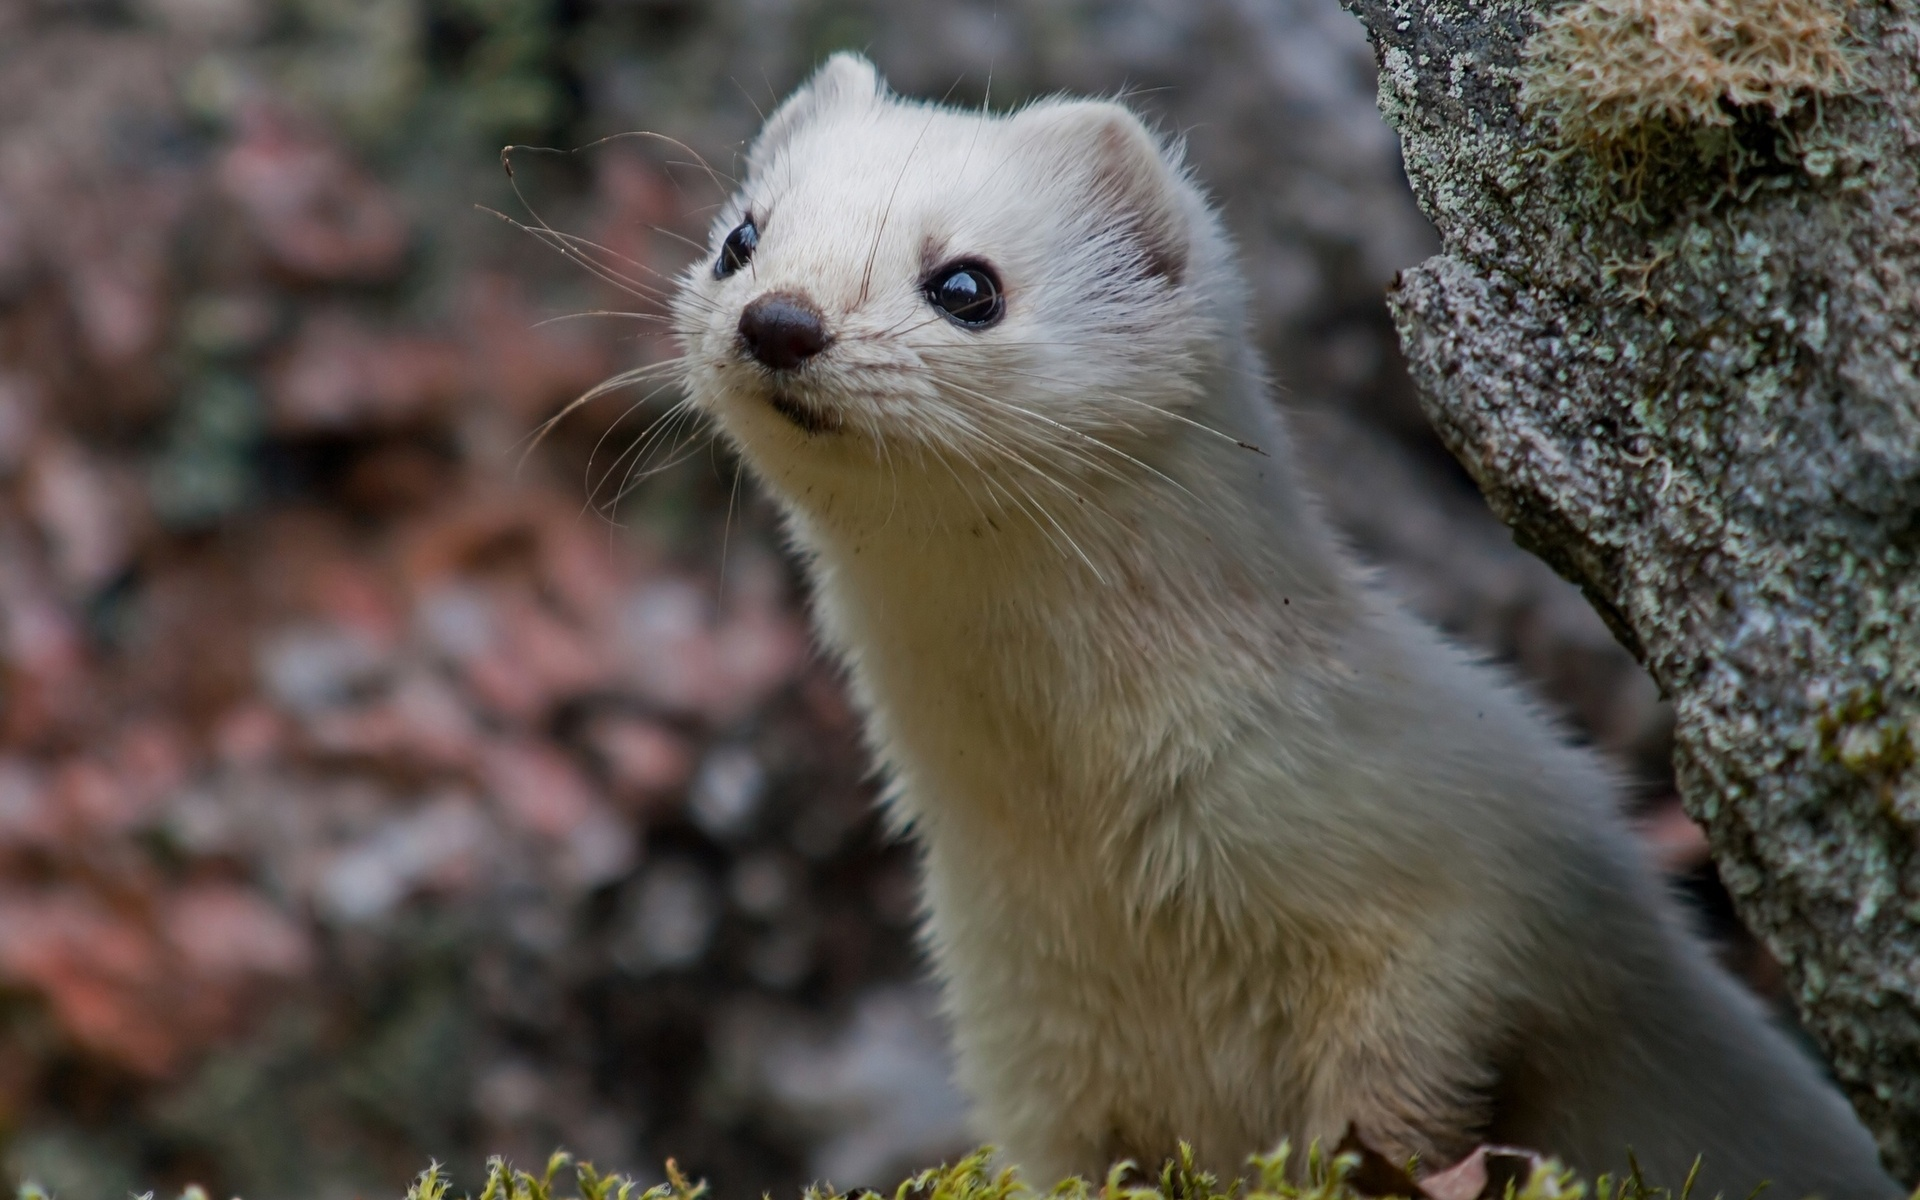
\includegraphics[width=.9\linewidth]{/Users/jay/Dropbox/github/org-html-webslides/assets/img/weasel.jpg}
\end{center}

\subsubsection[Notes]{Notes\hfill{}\textsc{notes}}
\label{sec:orgd3119d1}
Pop goes the weasel.

I'm just going to stop it right there.

How do you guys feel?

Hmm\ldots{}

\subsection[Mind Control]{Mind Control\hfill{}\textsc{slide:invisible:full}}
\label{sec:org16d0d61}
\begin{center}

\includegraphics[width=.9\linewidth]{/Users/jay/Dropbox/github/org-html-webslides/assets/img/videogame-brain-desire.png}
\end{center}


\subsection[This American Life: ``Cringe'']{This American Life: ``Cringe''\hfill{}\textsc{slide}}
\label{sec:orga762e5c}


\subsubsection[Notes]{Notes\hfill{}\textsc{notes}}
\label{sec:org4ca344e}
Let me give you another example.

Ira Glass, This American Life.
\subsection[\textbf{Nobody} turns off the radio at this point]{\textbf{Nobody} turns off the radio at this point\hfill{}\textsc{slide:aligncenter}}
\label{sec:org5f6afcf}
\textbf{Why?}

\subsubsection[Notes]{Notes\hfill{}\textsc{notes}}
\label{sec:orgd560e7f}
\textbf{QUESTION:} How do you guys feel?
Is that OK?
How do you feel?
You have a question you want ANSWERED.
An emotion.
\begin{itemize}
\item desire to know more
\end{itemize}
What is it you want to know?
And \textbf{WHERE} is all this happening?

\subsection[Writing with the customer in mind]{Writing with the customer in mind\hfill{}\textsc{slide:darkbloom}}
\label{sec:org08559bc}
\begin{center}
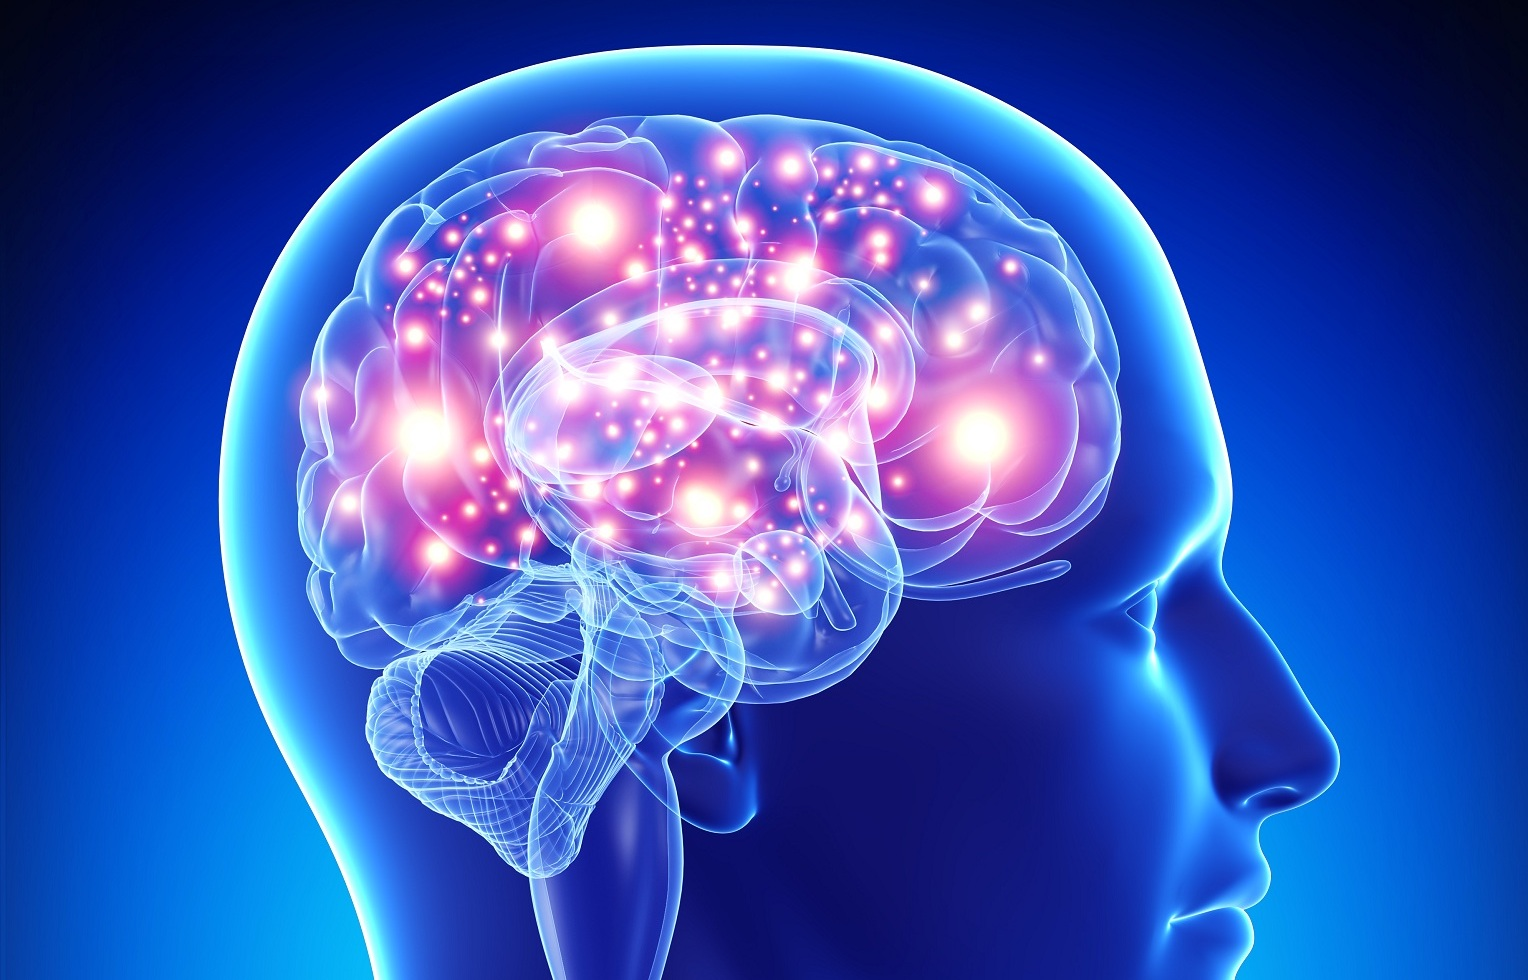
\includegraphics[width=.9\linewidth]{/Users/jay/Dropbox/github/org-html-webslides/assets/img/mind02.jpg}
\end{center}

\subsubsection[Notes]{Notes\hfill{}\textsc{notes}}
\label{sec:orgdbd0dab}
\textbf{WHERE} is all this happening?

In the mind of the listener.

That's when I want to start to do is to give you guys some habits for writing with the customer in mind.

Thinking about the MIND of the prospect while you're writing.

OK so let's recap. What's the fact pattern so far?

What do we know? Where does this take place?
\subsection[Hallway]{Hallway\hfill{}\textsc{slide:full:invisible}}
\label{sec:org3f6bfe8}
\begin{center}
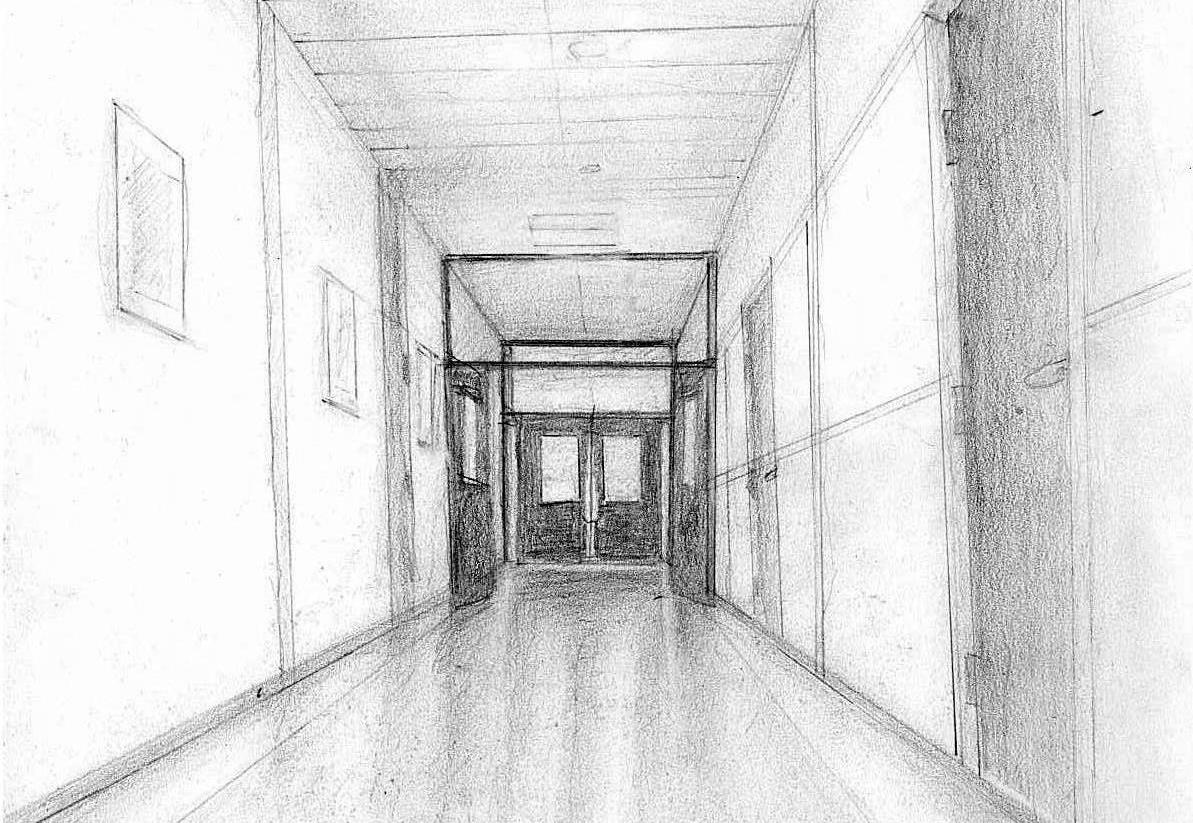
\includegraphics[width=.9\linewidth]{/Users/jay/Dropbox/github/org-html-webslides/assets/img/hallway.jpg}
\end{center}

\subsubsection[Notes]{Notes\hfill{}\textsc{notes}}
\label{sec:org53b888d}
OK so there's a hallway\ldots{}

What's special?

Everything is not as it seems\ldots{}

\subsection[No glasses]{No glasses\hfill{}\textsc{slide:full:invisible}}
\label{sec:org56fa5c6}
\begin{center}
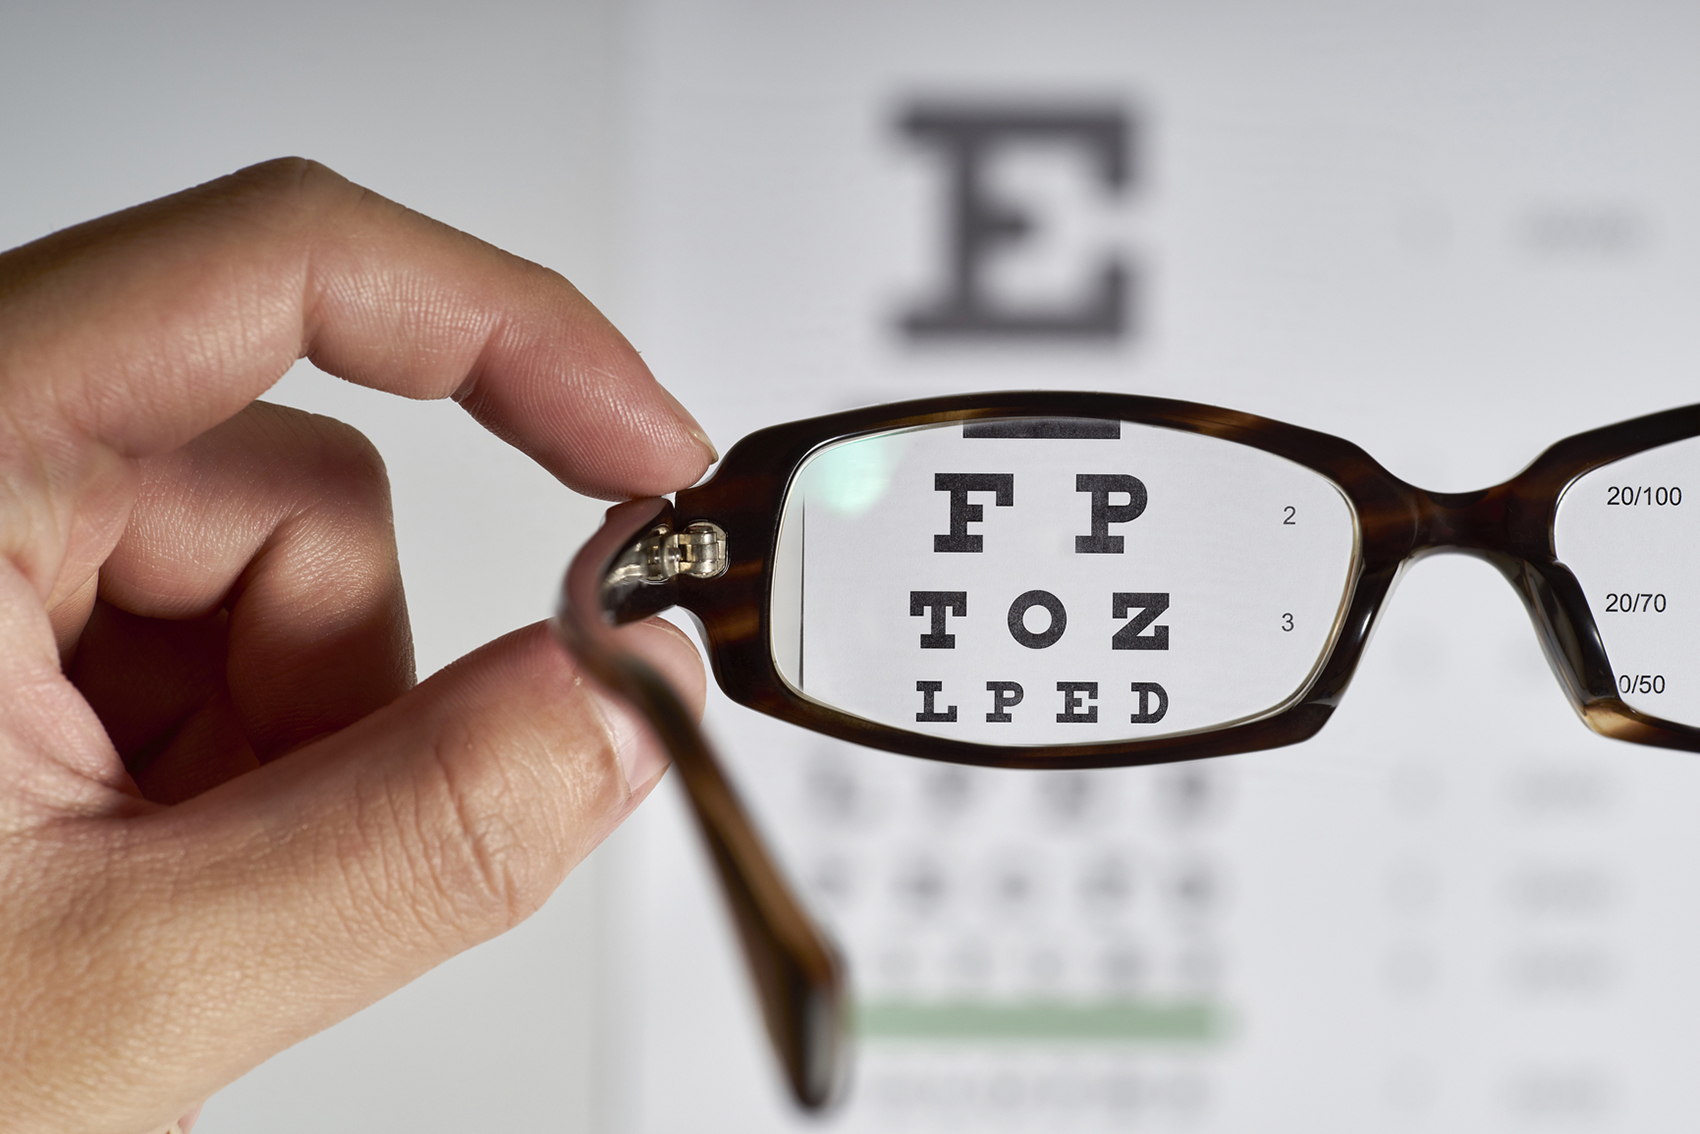
\includegraphics[width=.9\linewidth]{/Users/jay/Dropbox/github/org-html-webslides/assets/img/glasses-vision.jpg}
\end{center}

\subsubsection[Notes]{Notes\hfill{}\textsc{notes}}
\label{sec:org5d037b8}
The detail: he's not wearing his glasses!!!

\subsection[Blurry hallway]{Blurry hallway\hfill{}\textsc{slide:full:invisible}}
\label{sec:org3e5d91f}
\begin{center}

\includegraphics[width=.9\linewidth]{/Users/jay/Dropbox/github/org-html-webslides/assets/img/hallway-blurry.gif}
\end{center}

\subsubsection[Notes]{Notes\hfill{}\textsc{notes}}
\label{sec:org666ba5e}
OK so he can't see\ldots{}

What's the question we want to know the answer to?

YES! WHO is it?

You guys want to hear the rest?

\subsection[This American Life: ``Cringe,'' Part Two]{This American Life: ``Cringe,'' Part Two\hfill{}\textsc{slide}}
\label{sec:orgbef2ade}

\subsection[\textbf{Writing} with the customer \textbf{in mind}]{\textbf{Writing} with the customer \textbf{in mind}\hfill{}\textsc{slide}}
\label{sec:orgabbf750}

\subsubsection[Notes]{Notes\hfill{}\textsc{notes}}
\label{sec:orge969856}

\subsection[Writing with the reader in mind]{Writing with the reader in mind\hfill{}\textsc{slide:darkbloom}}
\label{sec:org02d4698}
\begin{center}
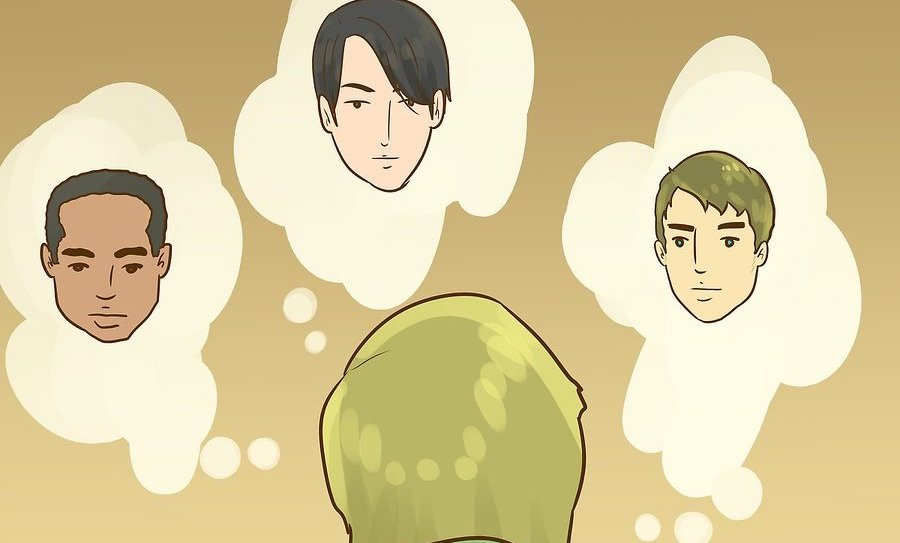
\includegraphics[width=.9\linewidth]{/Users/jay/Dropbox/github/org-html-webslides/assets/img/writing-with-the-reader-in-mind-crop.jpg}
\end{center}

\subsection[Effective response emails]{Effective response emails\hfill{}\textsc{slides}}
\label{sec:orga15084d}

\subsubsection[Notes]{Notes\hfill{}\textsc{notes}}
\label{sec:org956f21d}
I've had a chance to look over your emails

I think there are opportunities to craft emails that are going to have the outcome that we're after.

So what is that outcome? What are our objectives?

and we're going to focus on one of these today

\subsection[Objectives]{Objectives\hfill{}\textsc{slide}}
\label{sec:org5e7cf9e}
\subsubsection[Notes]{Notes\hfill{}\textsc{notes}}
\label{sec:org8e8ed5d}
What are the objectives in responding to an email?

(Don't give away the framework here.)

\textbf{Objective:} We'll learn how to write emails that get responses.

What's the objective of a sales email response?

\subsection[Examples]{Examples\hfill{}\textsc{slide}}
\label{sec:orgcae7a15}

\subsubsection[Notes]{Notes\hfill{}\textsc{notes}}
\label{sec:org9edae31}
I want us to start by looking at a counterexample.

Franken-email based on various emails.

You all have strengths and weaknesses,

\subsection[An inquiry about D\&I]{An inquiry about D\&I\hfill{}\textsc{slide}}
\label{sec:org6394860}

\begin{quote}
My name is Ellen. We haven't met but a colleague recommended I speak to you, she had worked with you before and suggested you might be able to help us think about our overall D \& I strategy. What is your approach to D \& I and unconscious bias? We are a technology and media company with offices in 20 countries and around 60,000 employees, and I look after HR and talent. Our HQ is based in Philadelphia.

Ellen Page
VP of Human Resources
Sanfino Corporation
\end{quote}

\subsection[Sample response]{Sample response\hfill{}\textsc{slide}}
\label{sec:org7efe514}

\begin{quote}
Hello,

Hope you are doing well.

The NeuroLeadership Institute has operations in 24 countries and our content and frameworks have been designed for a global audience. D\&I is an area which we have been heavily invested in over the last year and a half now and we've already been making major inroads in the market.

In regard to D\&I, the benefits derived from diverse teams have become
increasingly clear (\href{https://hbr.org/2016/11/why-diverse-teams-are-smarter}{click here} to learn more). NLI tackles this piece by stressing the importance of team coherence. While conventional wisdom says homogeneous teams create the best work, research has uncovered that it is actually heterogeneous teams that live on the cutting-edge of innovation though they may be more difficult to navigate. Therefore, it is important for organizations to facilitate inclusive teams to bring out the best of each teammate.

NLI's approach revolves around utilizing our SCARF model to alleviate interpersonal tension, minimizing what we call, the threat state. Research shows that when we are threatened, our brains shut down and cannot properly process information (threat elicits the fight-or-flight response). When we feel safe in a social situation, or are in what we call a toward state, we think clearer and are open to ideas and collaboration.

For your review, I have attached an article from s+b (Managing With the Brain in Mind) to this email. While this article is not directly tied to our inclusion work, it clearly outlines the research foundation for the SCARF model and will be helpful in framing our approach.

After you review the material sent here, we can schedule a meeting with our Senior Consultant for Performance management to answer any questions or concerned you may have.

I will circle back with you in the next couple of days with some time availability to offer more insights that can help you with the challenges you and your team might be facing around your D\&I strategy.

Please let me know what works best for you as I am happy to coordinate.
\end{quote}

\subsubsection[Notes]{Notes\hfill{}\textsc{notes}}
\label{sec:orge934131}
READ COUNTEREXAMPLE

\begin{enumerate}
\item Let's take a look at it and why it isn't working
\item They'll say qualities
\item I chart it up
\end{enumerate}

\subsection[A different approach]{A different approach\hfill{}\textsc{slide}}
\label{sec:org1aeec36}
\begin{quote}
Hi Ellen,

Good to hear from you, and thank you so much for reaching out. Absolutely, I'd be more than happy to talk about how NLI can help you with your D\&I strategy.

As you think about how to address D\&I at Sanfino, I'll start by saying I think this is a really tricky challenge. \href{//hbr.org/2016/07/why-diversity-programs-fail}{Most D\&I programs fail} because they focus on trying to make individuals less biased, which doesn't work because bias is unconscious. At NLI, we focus instead on taking the bias out of \textbf{decisions,} teaching organizations how to structure processes so as to sidestep the pitfalls of our biased brains.

So far we've helped improve decision making at 40 companies, including \href{https://neuroleadership.com/portfolio-items/case-study-blackrock-breaking-bias/}{BlackRock} and \href{https://neuroleadership.com/portfolio-items/nli-transforms-intel-culture/}{Intel}, and most of our clients still use our tools at least once a week.

I'd love to set up a time to talk on the phone so I can hear more about your objectives. I'm available for a quick call at the following times:

\begin{itemize}
\item Monday Oct 6, 1:00pm
\item Wednesday Oct 8, 4:00pm
\item Friday Oct 10, 9:00am
\end{itemize}

Do any of those times work for you?

I look forward to connecting!

Best, \\
Jay
\end{quote}

\subsubsection[Notes]{Notes\hfill{}\textsc{notes}}
\label{sec:org43f8315}
\begin{itemize}
\item Discuss how/why the mentor text is better
\item Chart what they say
\item Look for connections to my framework
\end{itemize}

\subsection[Writing with the reader in mind]{Writing with the reader in mind\hfill{}\textsc{slide}}
\label{sec:org6fdf9e5}

\subsection[\textbf{3 QUALITIES} of an effective response email]{\textbf{3 QUALITIES} of an effective response email\hfill{}\textsc{slide:wrap:size60:bgwhite:shadow:flexblock:reasons:fancynumberedlist}}
\label{sec:org5920881}

\subsection[\textbf{3 QUALITIES} of an effective response email]{\textbf{3 QUALITIES} of an effective response email\hfill{}\textsc{slide:wrap:size60:bgwhite:shadow:flexblock:reasons:fancynumberedlist:invisible}}
\label{sec:org4bdefa7}
\begin{enumerate}
\item *Relevant*t \begin{center}

\includegraphics[width=.9\linewidth]{/Users/jay/Dropbox/github/org-html-webslides/assets/img/noun_502032_cc.png}
\end{center}
\item \textbf{Personal} \begin{center}

\includegraphics[width=.9\linewidth]{/Users/jay/Dropbox/github/org-html-webslides/assets/img/flamenco-couple-dance_318-56562.jpg}
\end{center}
\item \textbf{Persuasive} \begin{center}

\includegraphics[width=.9\linewidth]{/Users/jay/Dropbox/github/org-html-webslides/assets/img/smoker-004-512.png}
\end{center}
\end{enumerate}
\subsubsection[Notes]{Notes\hfill{}\textsc{notes}}
\label{sec:orgc232669}
In each session we'll discuss one of these qualities and how we can develop these qualities in our own emails

\subsection[\textbf{3 QUALITIES} of an effective response email]{\textbf{3 QUALITIES} of an effective response email\hfill{}\textsc{slide}}
\label{sec:org605b97d}
\begin{enumerate}
\item *Relevant*t \begin{center}

\includegraphics[width=.9\linewidth]{/Users/jay/Dropbox/github/org-html-webslides/assets/img/noun_502032_cc.png}
\end{center}
\item \textbf{Personal} \begin{center}

\includegraphics[width=.9\linewidth]{/Users/jay/Dropbox/github/org-html-webslides/assets/img/flamenco-couple-dance_318-56562.jpg}
\end{center}
\item \textbf{Persuasive} \begin{center}

\includegraphics[width=.9\linewidth]{/Users/jay/Dropbox/github/org-html-webslides/assets/img/smoker-004-512.png}
\end{center}
\end{enumerate}
\subsubsection[Notes]{Notes\hfill{}\textsc{notes}}
\label{sec:org565732d}
In each session we'll discuss one of these qualities and how we can develop these qualities in our own emails

\subsection[\textbf{RELEVANCE}]{\textbf{RELEVANCE}\hfill{}\textsc{slide}}
\label{sec:org339d8a1}
\begin{center}

\includegraphics[width=.9\linewidth]{/Users/jay/Dropbox/github/org-html-webslides/assets/img/noun_502032_cc.png}
\end{center}

\subsubsection[Notes]{Notes\hfill{}\textsc{notes}}
\label{sec:orgb44830b}

Today we're going to focus on \textbf{relevance}.

\subsection[\textbf{EMPATHY}]{\textbf{EMPATHY}\hfill{}\textsc{slide}}
\label{sec:org28e388b}

\subsubsection[Notes]{Notes\hfill{}\textsc{notes}}
\label{sec:org56a5dc3}
What does this mean in the context of sales?

\begin{itemize}
\item listening
\item understanding what they want
\item how they feel
\end{itemize}

\subsection[\textbf{EMPATHY}]{\textbf{EMPATHY}\hfill{}\textsc{slide}}
\label{sec:orgacf5886}



\subsubsection[Notes]{Notes\hfill{}\textsc{notes}}
\label{sec:orge587dc9}
What did Bill Clinton do differently?

\subsection[Put yourself in the shoes of the human being on the other end of your email]{Put yourself in the shoes of the human being on the other end of your email\hfill{}\textsc{slide}}
\label{sec:org0645c91}

\subsection[Theory of mind]{Theory of mind\hfill{}\textsc{slide:full:invisible}}
\label{sec:orge91894b}
\begin{center}
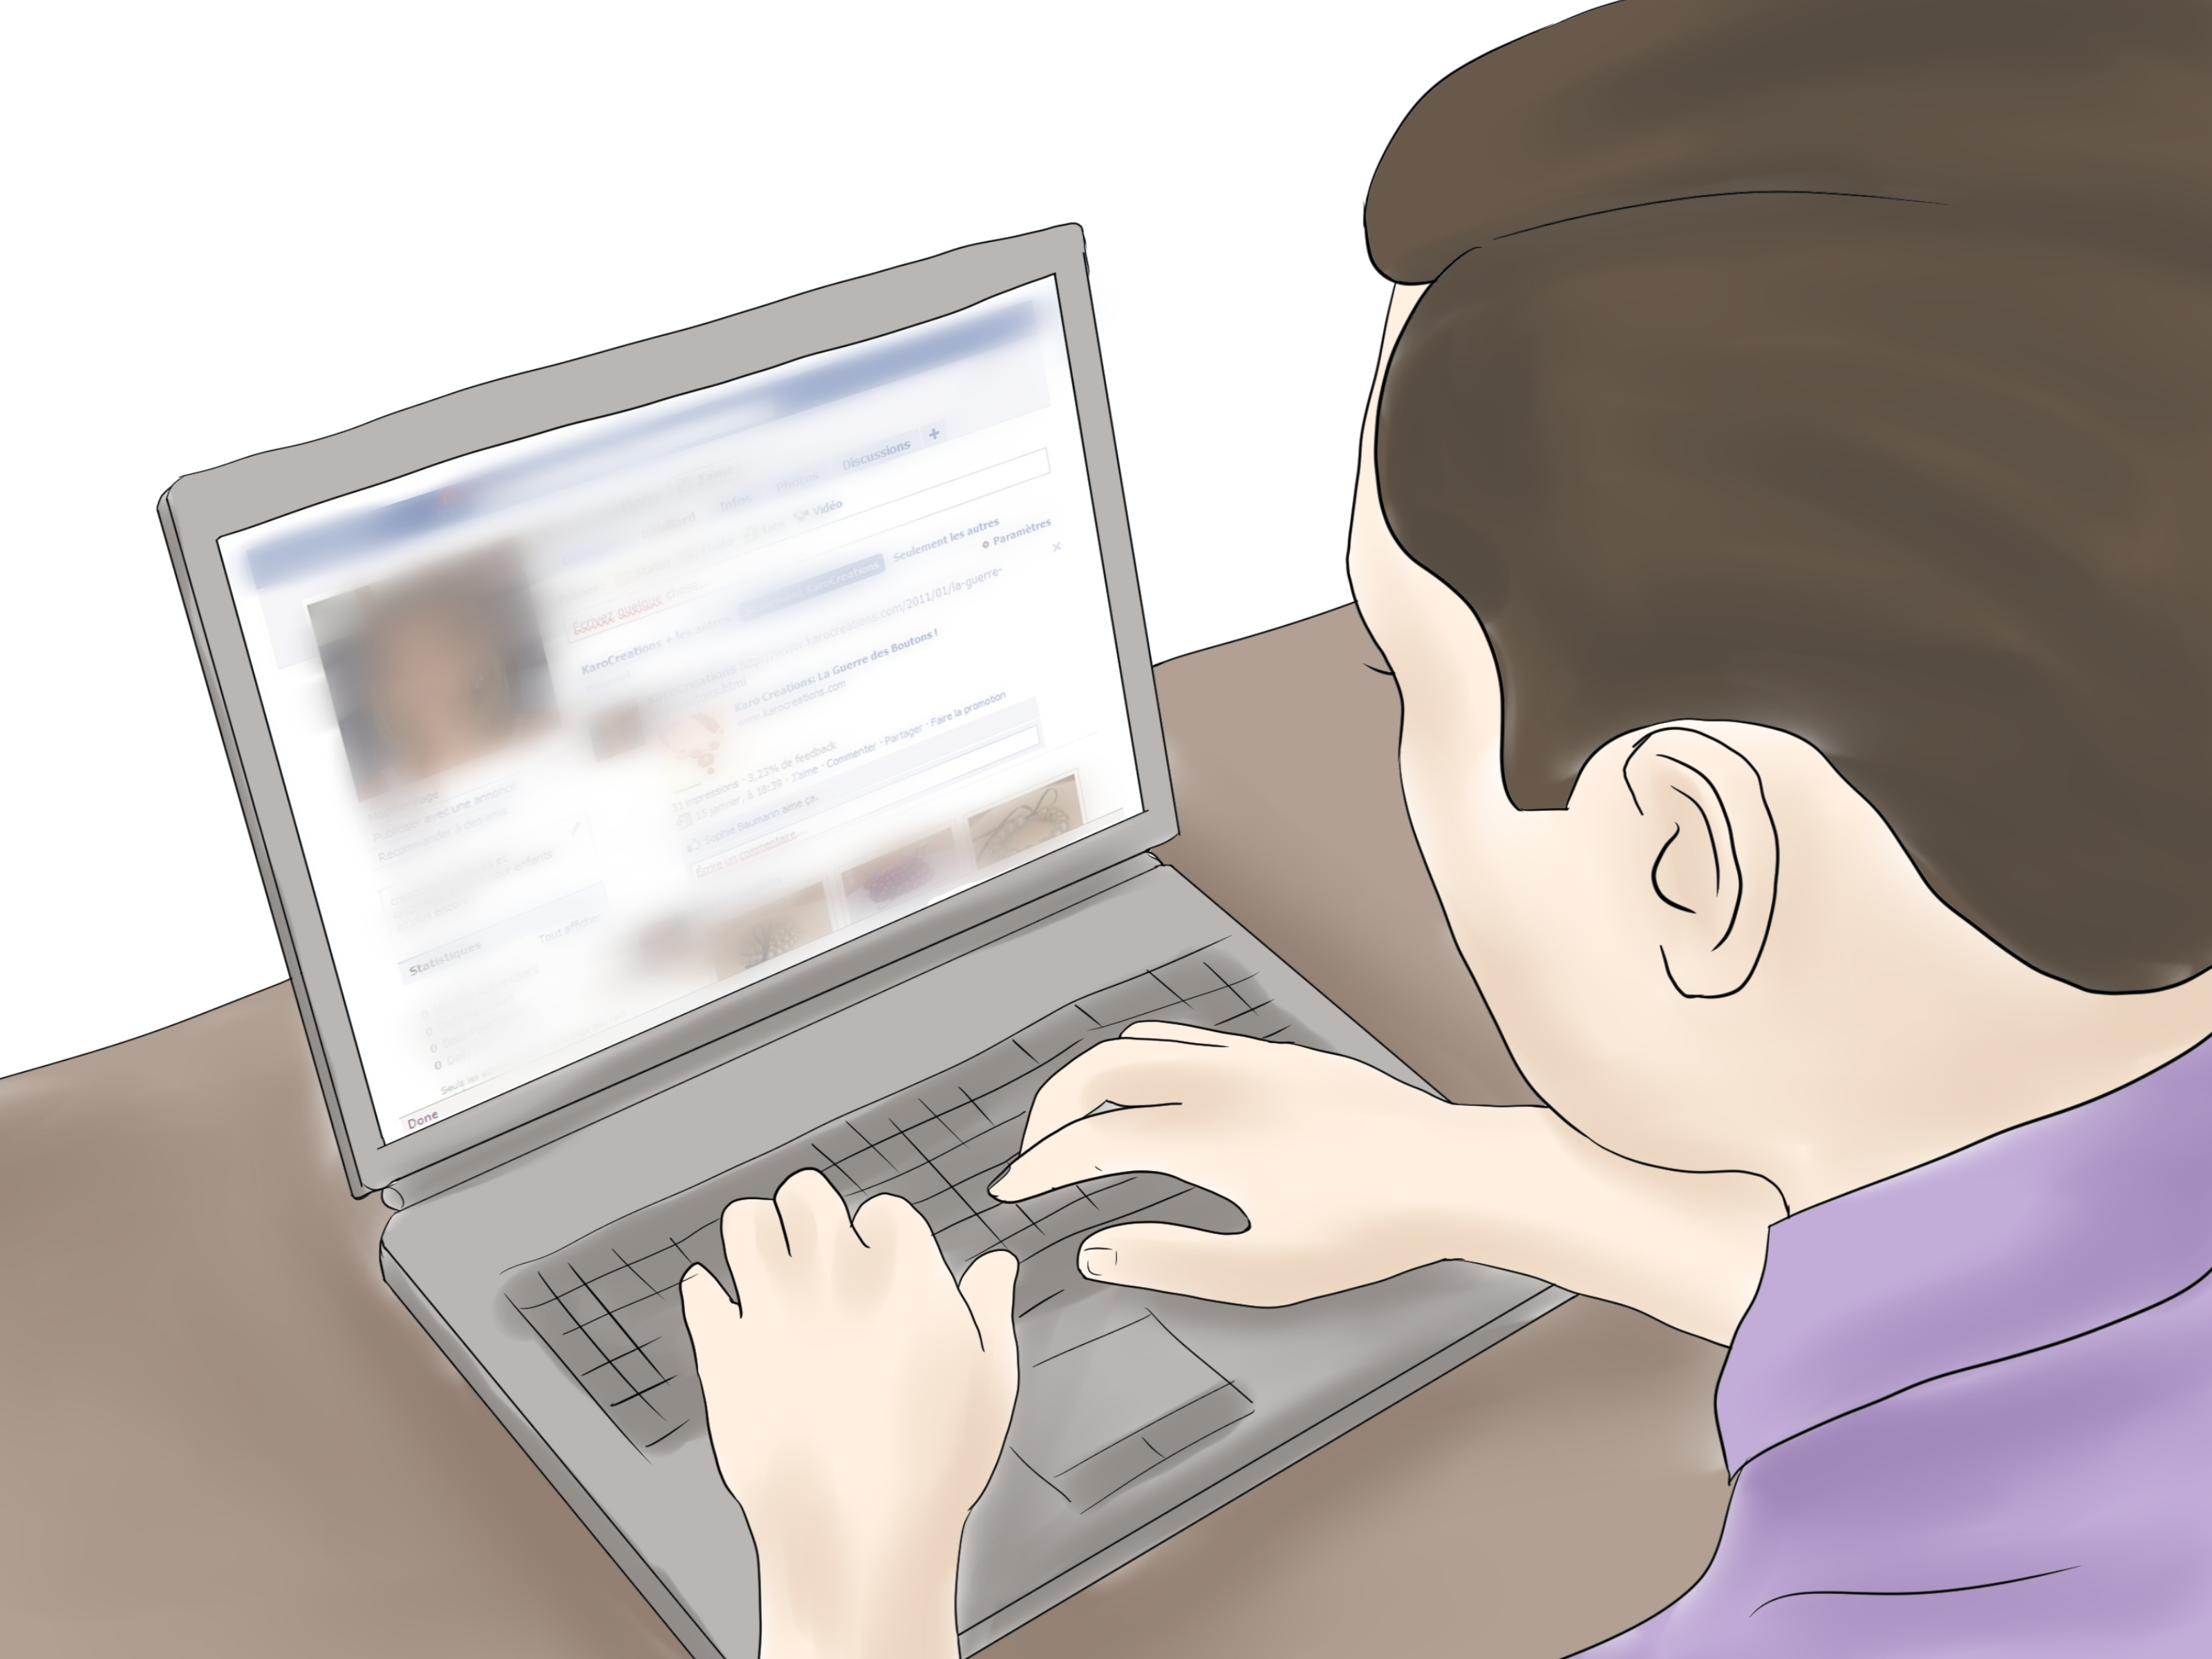
\includegraphics[width=.9\linewidth]{/Users/jay/Dropbox/github/org-html-webslides/assets/img/Buy-Laptops-in-Bulk-Step-9.jpg}
\end{center}

\subsubsection[Notes]{Notes\hfill{}\textsc{notes}}
\label{sec:orga064139}
\textbf{QUESTION:} What can you think about when you're responding to a sales email?

\begin{itemize}
\item What do they want?
\item What do they want to know?
\end{itemize}

\subsection[Theory of mind]{Theory of mind\hfill{}\textsc{slide:full:invisible}}
\label{sec:orge8352ee}
\begin{center}
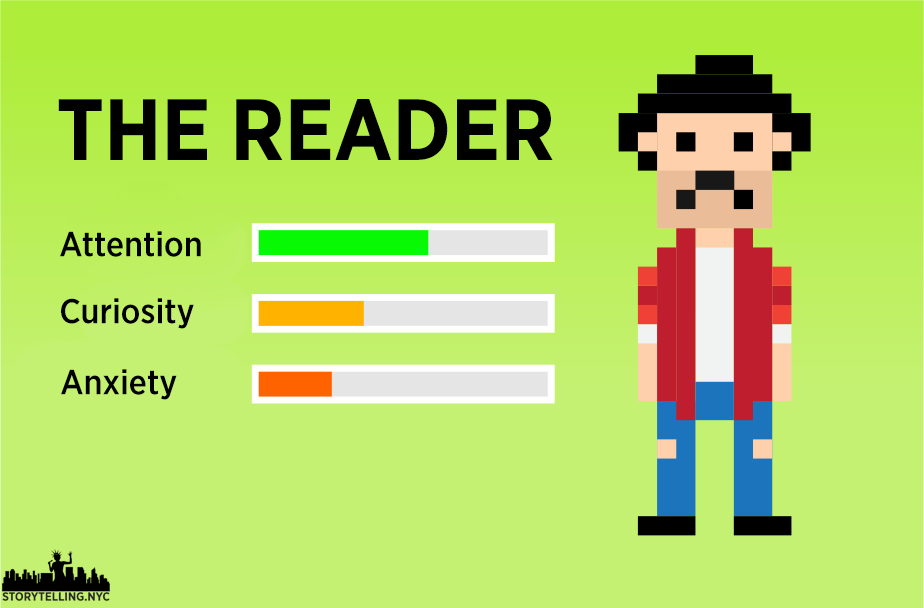
\includegraphics[width=.9\linewidth]{/Users/jay/Dropbox/github/org-html-webslides/assets/img/videogame-state-levels-theory-of-mind.png}
\end{center}

\subsubsection[Notes]{Notes\hfill{}\textsc{notes}}
\label{sec:orgef216dd}
It helps to almost have an avatar of the reader in your mind

\begin{itemize}
\item What are the reader's \textbf{wants}
\item What does the reader know / not know
\item How does the reader feel
\end{itemize}

What's the psych term for this?
\begin{itemize}
\item theory of mind
\item mentalizing
\item perspective taking
\end{itemize}

\subsection[The Three R's of Relevance]{The Three R's of Relevance\hfill{}\textsc{slide:wrap:size60:bgwhite:shadow:flexblock:reasons:fancynumberedlist}}
\label{sec:org9b6c0fe}
\begin{enumerate}
\item \textbf{Responsive} Answers their question directly and explicitly.
\item \textbf{Relevant} To the prospect's situation and needs.
\item \textbf{Restrained} With no unnecessary information.
\end{enumerate}

\subsection[1. Responsive]{1. Responsive\hfill{}\textsc{slide}}
\label{sec:orgde89c2c}
\begin{itemize}
\item Answers their question directly and explicitly
\end{itemize}

\subsection[Responsive]{Responsive\hfill{}\textsc{slide:full:invisible}}
\label{sec:org9e13d8b}
\begin{center}

\includegraphics[width=.9\linewidth]{/Users/jay/Dropbox/github/org-html-webslides/assets/img/batman-answer-the-question.png}
\end{center}

\subsubsection[Notes]{Notes\hfill{}\textsc{notes}}
\label{sec:orgee45830}
\textbf{Answer:}
\begin{itemize}
\item what did they ask?
\item what do they actually need?
\end{itemize}

\textbf{QUESTION:} What happens if what you're telling them is relevant to their question, but they don't realize that it is? They don't realize it's actually answering their question?

\textbf{ANSWER:} That's just as bad as random nonsense.

If they don't know it's relevant, and why it's relevant, then it's meaningless to them.

\subsection[2. Relevant]{2. Relevant\hfill{}\textsc{slide}}
\label{sec:orgbcfbd17}
\begin{itemize}
\item Never provide information without making it clear why it's relevant to the prospect
\end{itemize}

\subsubsection[Notes]{Notes\hfill{}\textsc{notes}}
\label{sec:org99d5a20}
Never provide information without telling them why it's relevant to them.

If you're copy-pasting a bunch of info about NLI and our achievements, you're not writing with the reader in mind

Sound like you copy-pasted it from a Wikipedia article

The prospect should NEVER EVER be able to say ``wait why are they telling me this?''

SNEAK the information in in the context of answering their question. e.g. here's why I think we could help you

\subsection[Relevant]{Relevant\hfill{}\textsc{slide:full:invisible}}
\label{sec:orgaa0e530}
\begin{center}
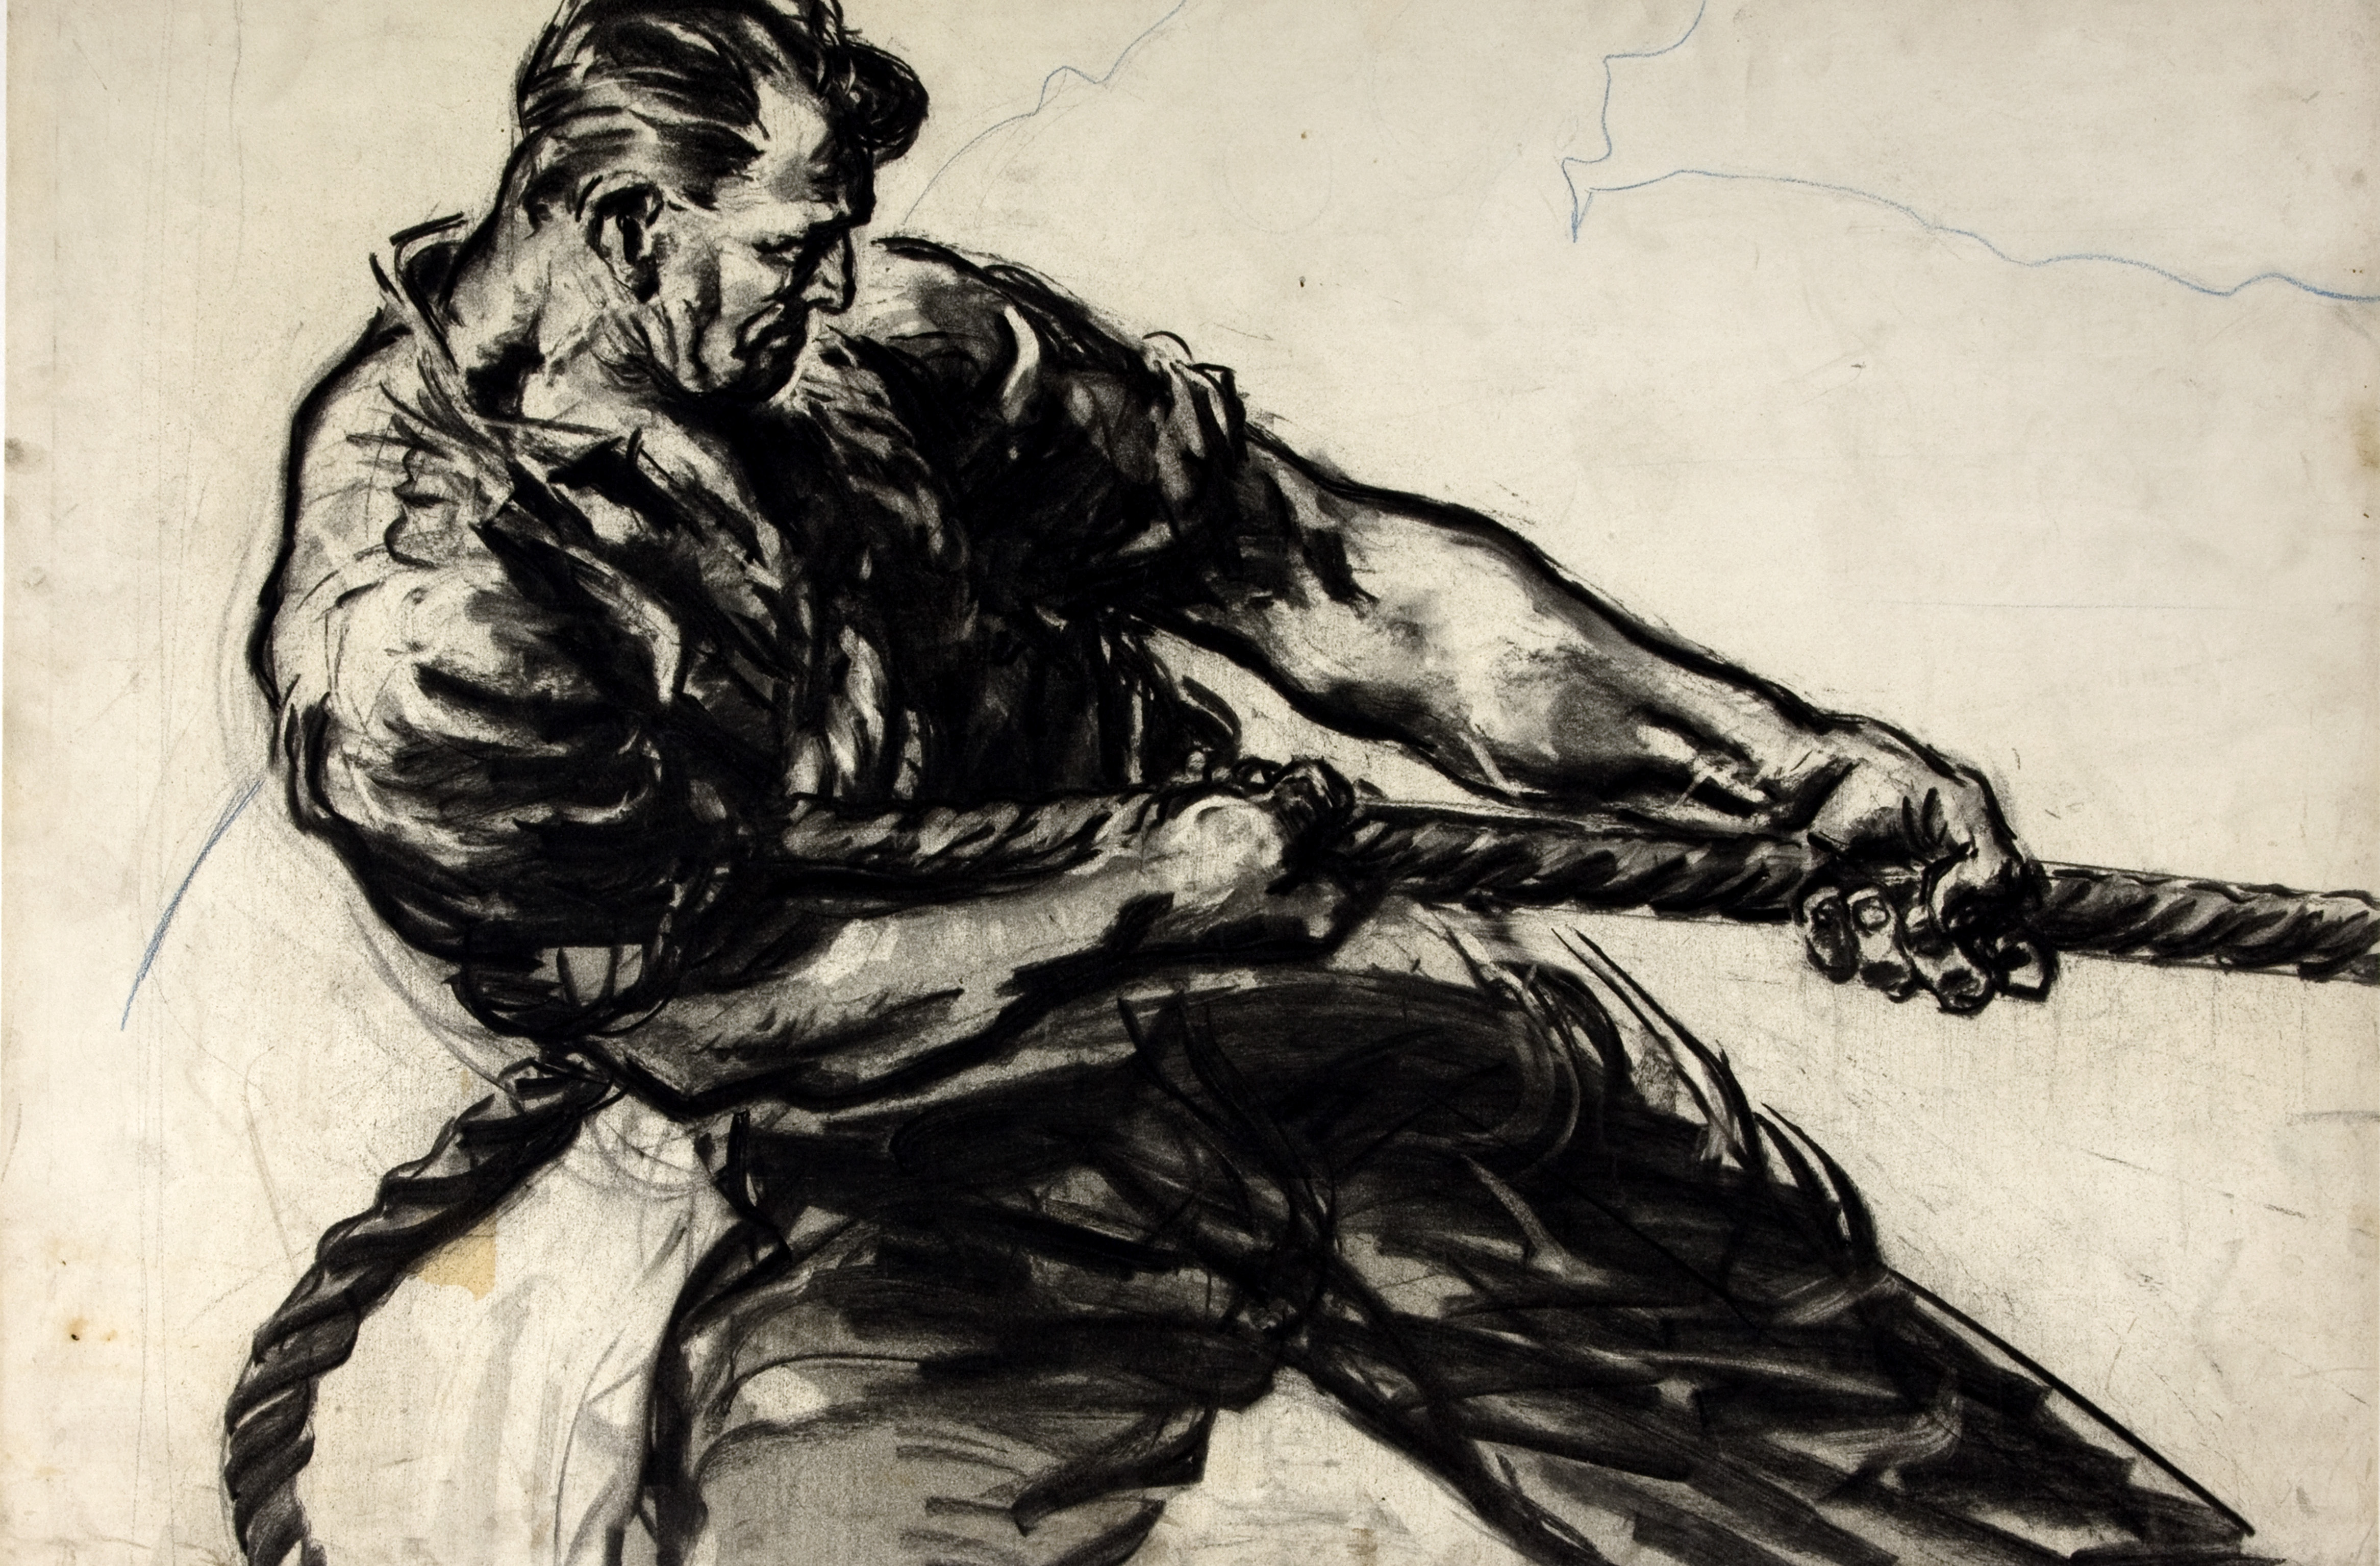
\includegraphics[width=.9\linewidth]{/Users/jay/Dropbox/github/org-html-webslides/assets/img/man_heaving_on_rope.png}
\end{center}

\subsubsection[Notes]{Notes\hfill{}\textsc{notes}}
\label{sec:org80ac82b}
Rope metaphor.

Don't let the rope go slack.

\subsection[3. Restrained]{3. Restrained\hfill{}\textsc{slide:aligncenter}}
\label{sec:orgf2cfc84}
\begin{itemize}
\item The prospect is on a need to know basis
\end{itemize}

\subsection[The prospect is on a need to know basis]{The prospect is on a need to know basis\hfill{}\textsc{slide:full:invisible}}
\label{sec:org159f75a}
\begin{center}
\includegraphics[width=.9\linewidth]{/Users/jay/Dropbox/storytelling-assets/need-to-know-basis.jpg}
\end{center}

\subsection[It's not about you.]{It's not about you.\hfill{}\textsc{slide}}
\label{sec:org8c57f92}
\begin{center}

\includegraphics[width=.9\linewidth]{/Users/jay/Dropbox/github/org-html-webslides/assets/img/kim_k_selfie.jpg}
\end{center}

\subsection[The Three R's of Relevance]{The Three R's of Relevance\hfill{}\textsc{slide:wrap:size60:bgwhite:shadow:flexblock:reasons:fancynumberedlist}}
\label{sec:org24428f3}
\begin{enumerate}
\item \textbf{Responsive} Answer the frickin' question.
\item \textbf{Relevant} Don't let the rope go slack.
\item \textbf{Restrained} It's not about you.
\end{enumerate}

\subsection[Mentor text analysis]{Mentor text analysis\hfill{}\textsc{slide}}
\label{sec:org5559c08}
\begin{quote}
Hi Ellen,

Good to hear from you, and thank you so much for reaching out. Absolutely, I'd be more than happy to talk about how NLI can help you with your D\&I strategy.

As you think about how to address D\&I at Sanfino, I'll start by saying I think this is a really tricky challenge. \href{//hbr.org/2016/07/why-diversity-programs-fail}{Most D\&I programs fail} because they focus on trying to make individuals less biased, which doesn't work because bias is unconscious. At NLI, we focus instead on taking the bias out of \textbf{decisions,} teaching organizations how to structure processes so as to sidestep the pitfalls of our biased brains.

So far we've helped improve decision making at 40 companies, including \href{https://neuroleadership.com/portfolio-items/case-study-blackrock-breaking-bias/}{BlackRock} and \href{https://neuroleadership.com/portfolio-items/nli-transforms-intel-culture/}{Intel}, and most of our clients still use our tools at least once a week.

I'd love to set up a time to talk on the phone so I can hear more about your objectives. I'm available for a quick call at the following times:

\begin{itemize}
\item Monday Oct 6, 1:00pm
\item Wednesday Oct 8, 4:00pm
\item Friday Oct 10, 9:00am
\end{itemize}

Do any of those times work for you?

I look forward to connecting!

Best, \\
Jay
\end{quote}

\subsubsection[Notes]{Notes\hfill{}\textsc{notes}}
\label{sec:org55d6da1}
Go back to the mentor text and focus in one just one of the qualities. Relevance. What are the \textbf{techniques} the writer used to make their email relevant?

Have them work in partners.

\subsection[Writing the relevant response email]{Writing the relevant response email\hfill{}\textsc{slide}}
\label{sec:orgd3313bb}

\subsubsection[Notes]{Notes\hfill{}\textsc{notes}}
\label{sec:org491b24e}
On your own, do the assignment.

\subsection[Yet to come\ldots{}]{Yet to come\ldots{}\hfill{}\textsc{slide:size60}}
\label{sec:orgc7a7f8c}

\textbf{Effective response emails}
\begin{itemize}
\item relevant
\item personal
\item persuasive
\end{itemize}

\textbf{Writing engaging sentences}
\begin{itemize}
\item simple and sticky
\item how to use visualness to lead the prospect's imagination
\item editing for concision
\end{itemize}

\textbf{Effective outgoing emails}
\begin{itemize}
\item subject headers that hook prospects and make them open
\item opening lines that draw prospects in and make them reply
\end{itemize}

\textbf{Strategy across the sales cycle}
\begin{itemize}
\item writing compelling opening emails to get the relationship on track for the sales cycle
\item writing effective follow-up emails: telling a story over the course of a series of emails
\item relating the story: strategy you use in email with the story you tell on sales calls
\end{itemize}


\subsection[Homework]{Homework\hfill{}\textsc{slide}}
\label{sec:org4cbaa4c}

\begin{center}

\includegraphics[width=.9\linewidth]{/Users/jay/Dropbox/github/org-html-webslides/assets/img/noun_1166730_cc.png}
\end{center}

\begin{enumerate}
\item \textbf{Collect examples of emails that display the qualities we've discussed---ideally, in an email you write in the next week.}
\item \textbf{Alternatively, take a past email and revise it to make it better.}
\end{enumerate}


\subsubsection[Notes]{Notes\hfill{}\textsc{notes}}
\label{sec:orgf217344}
\textbf{Homework:} collect real examples of what we just talked about. In an email you write in the next week ideally.

\textbf{Alternatively:} Take a paragraph of a past email you wrote and revise it to make it better.

\subsection[Q\&A]{Q\&A\hfill{}\textsc{slide}}
\label{sec:org38173c2}

\subsection{a few ways to create curiosity}
\label{sec:org6a57bd1}
(There are many others)

\subsection[Headlines]{Headlines\hfill{}\textsc{slide}}
\label{sec:orge64e6ab}
\begin{center}
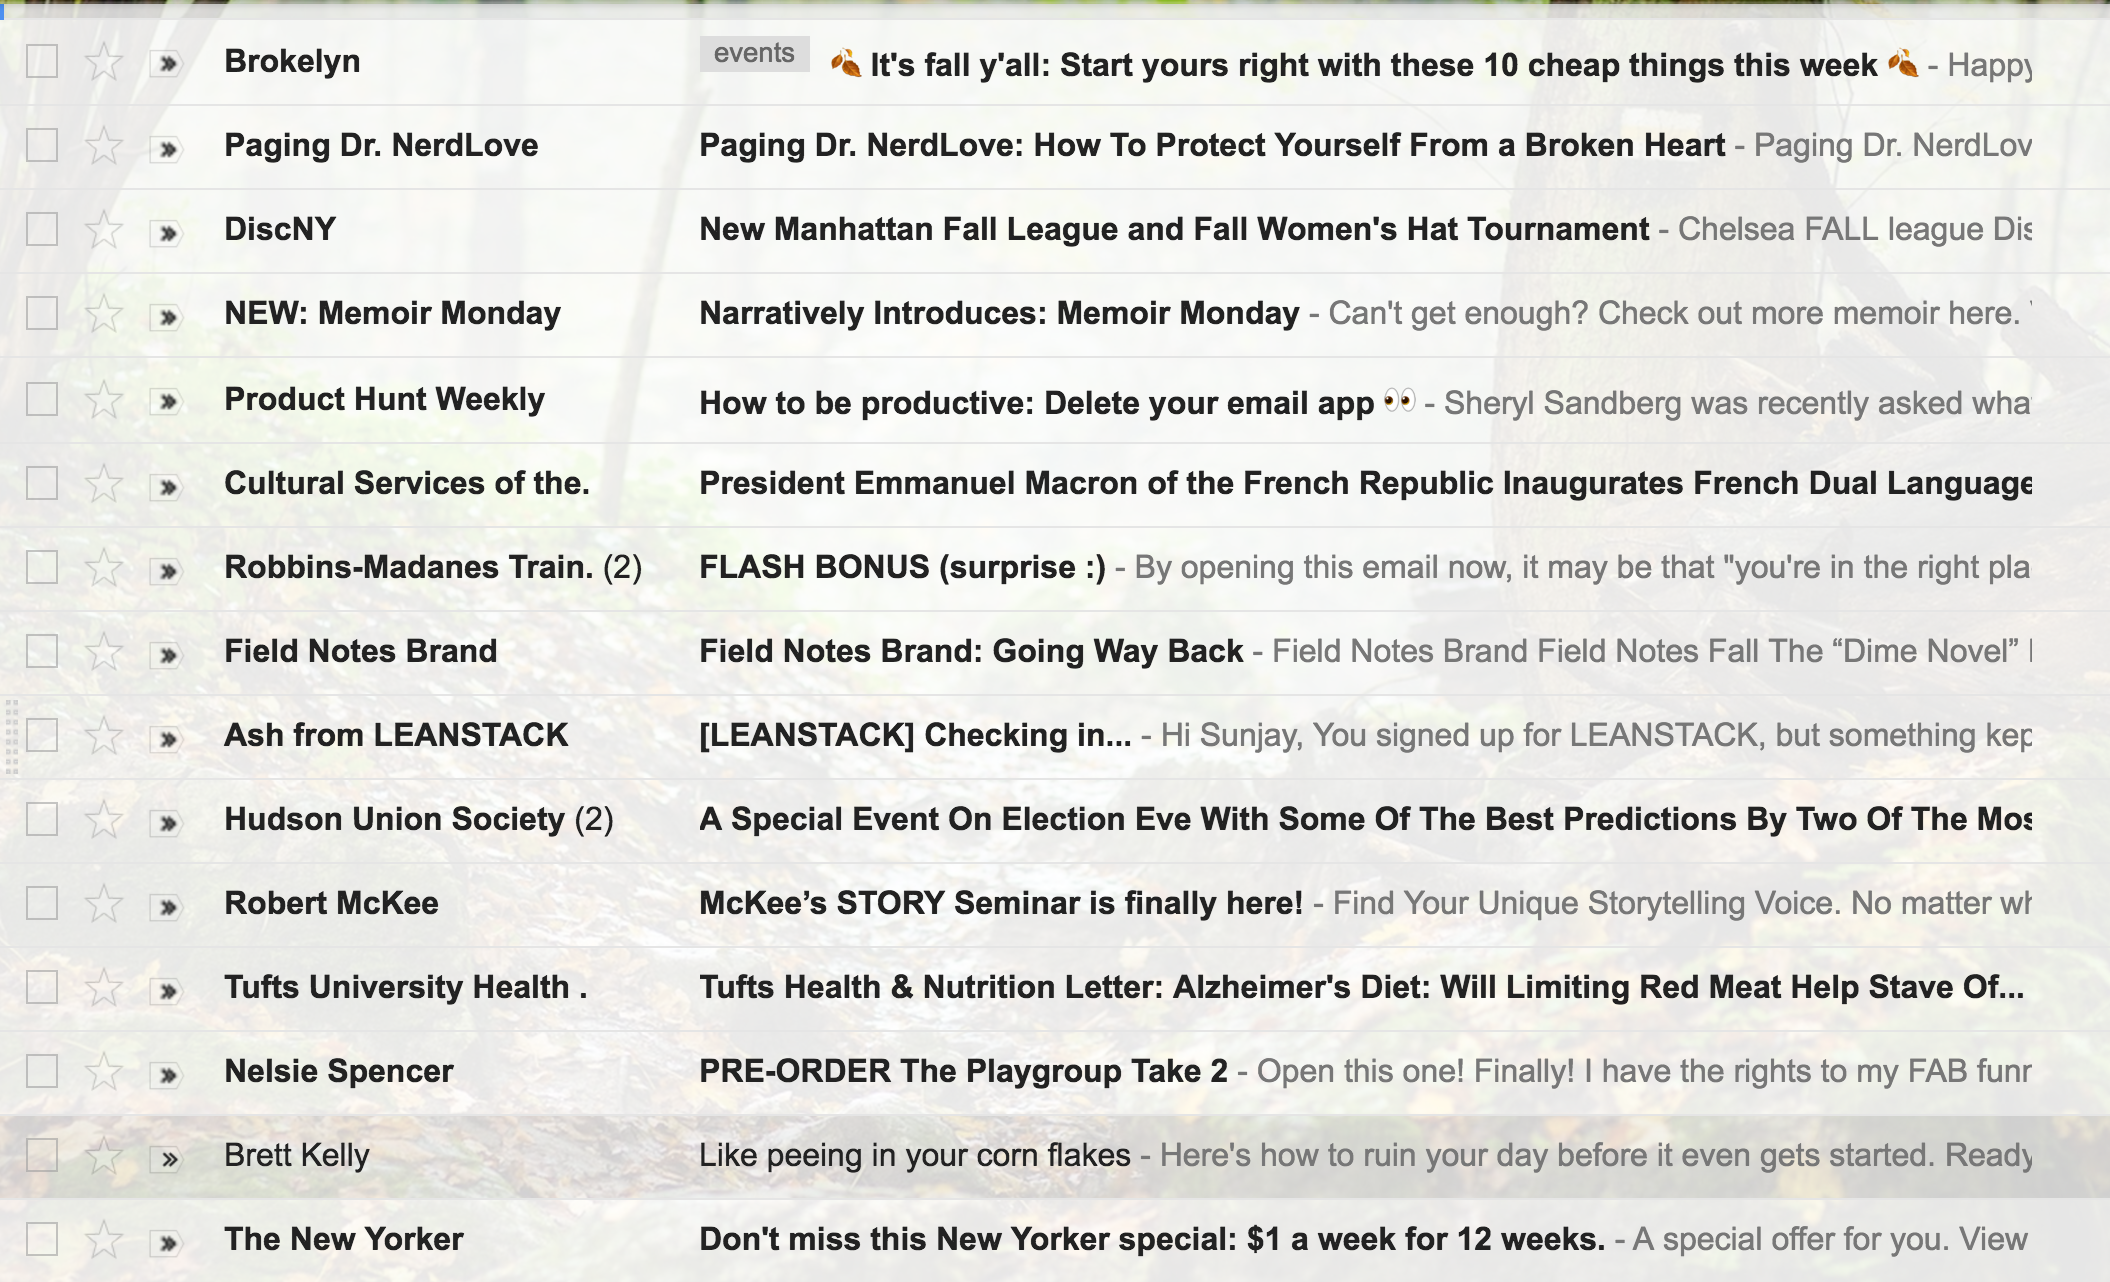
\includegraphics[width=.9\linewidth]{/Users/jay/Dropbox/github/org-html-webslides/assets/img/peeing-cornflakes.png}
\end{center}

\subsection[Headlines]{Headlines\hfill{}\textsc{slide}}
\label{sec:org6e7af1c}
\begin{center}
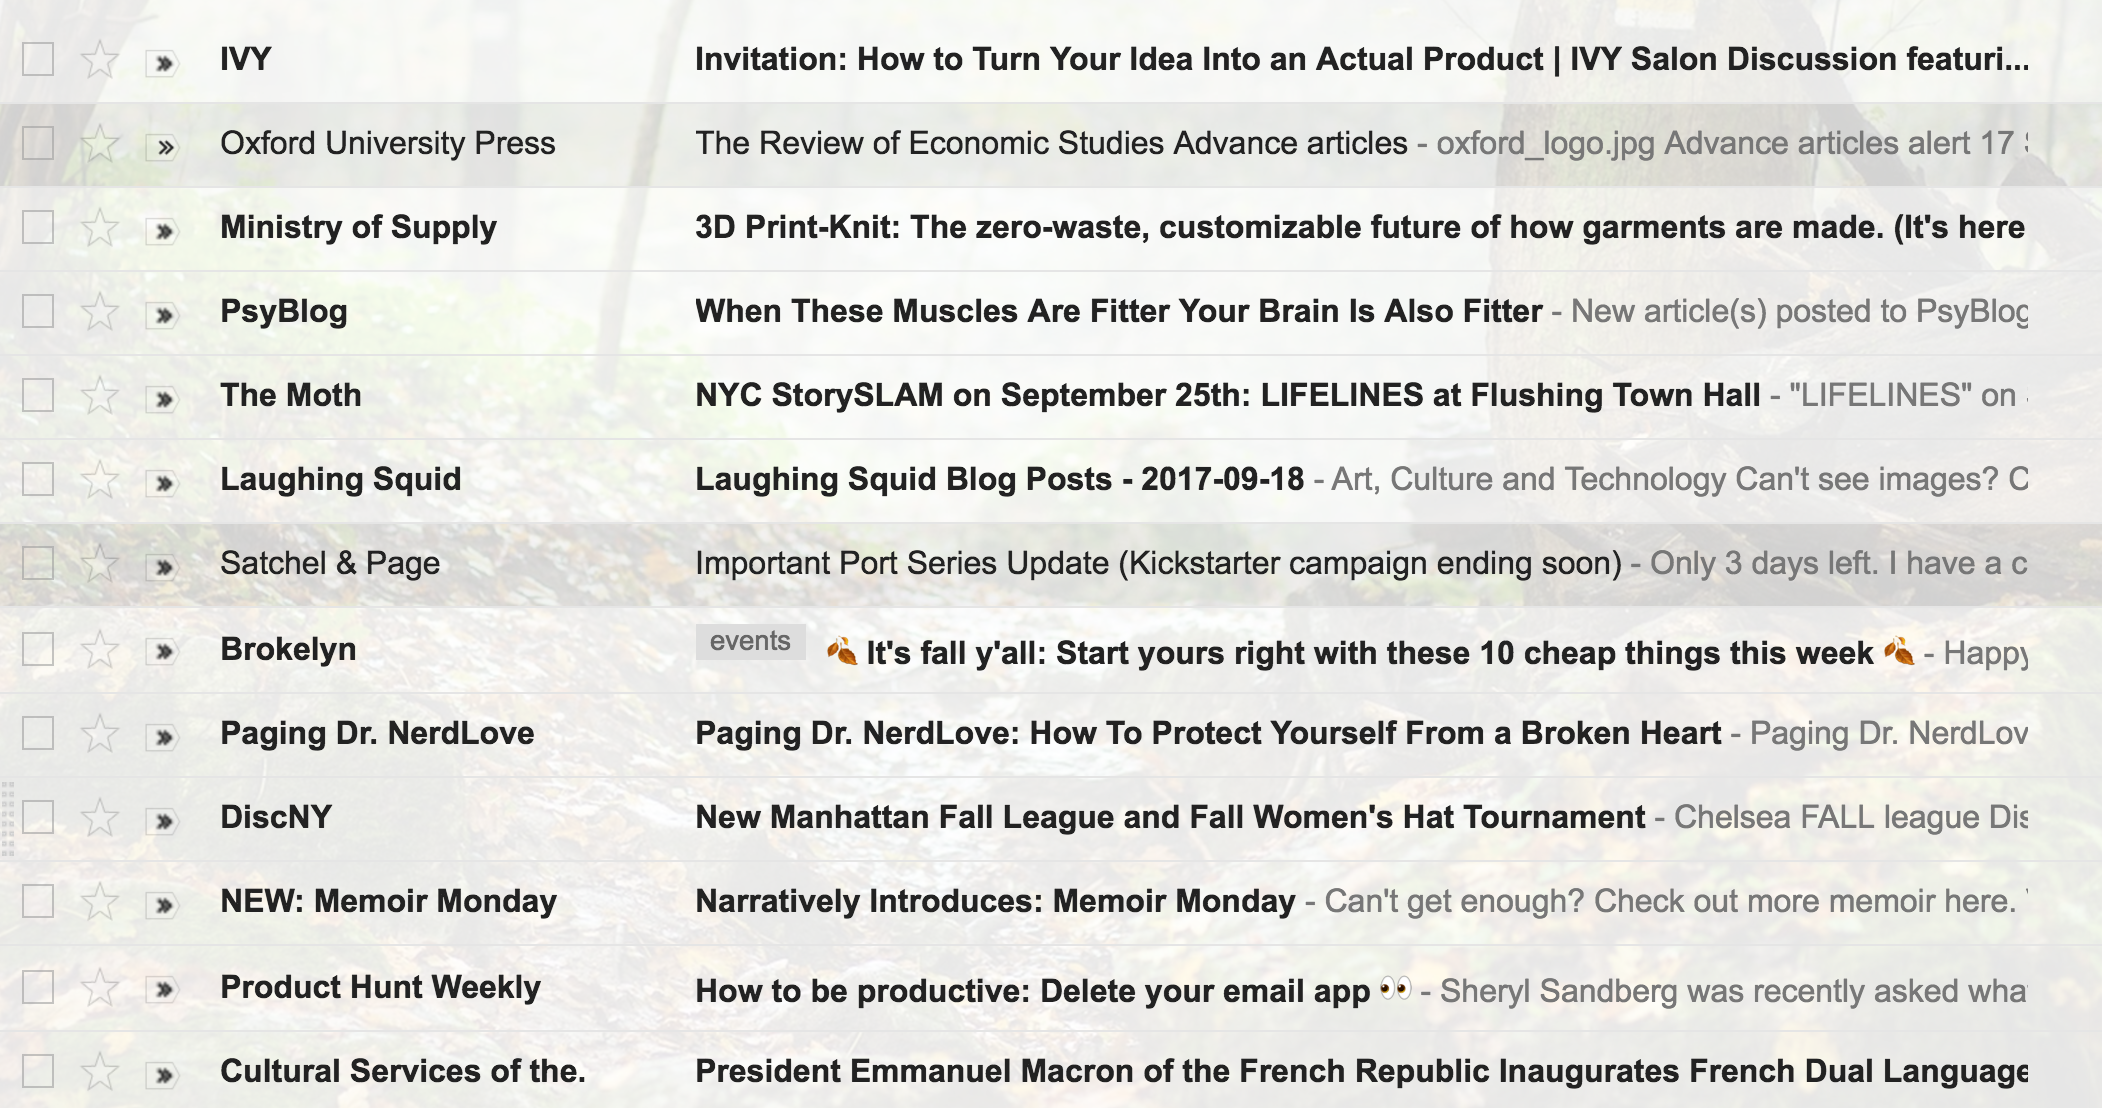
\includegraphics[width=.9\linewidth]{/Users/jay/Dropbox/github/org-html-webslides/assets/img/memoir-monday.png}
\end{center}


\subsection[Headlines]{Headlines\hfill{}\textsc{slide}}
\label{sec:orgcf5a10c}
\begin{center}
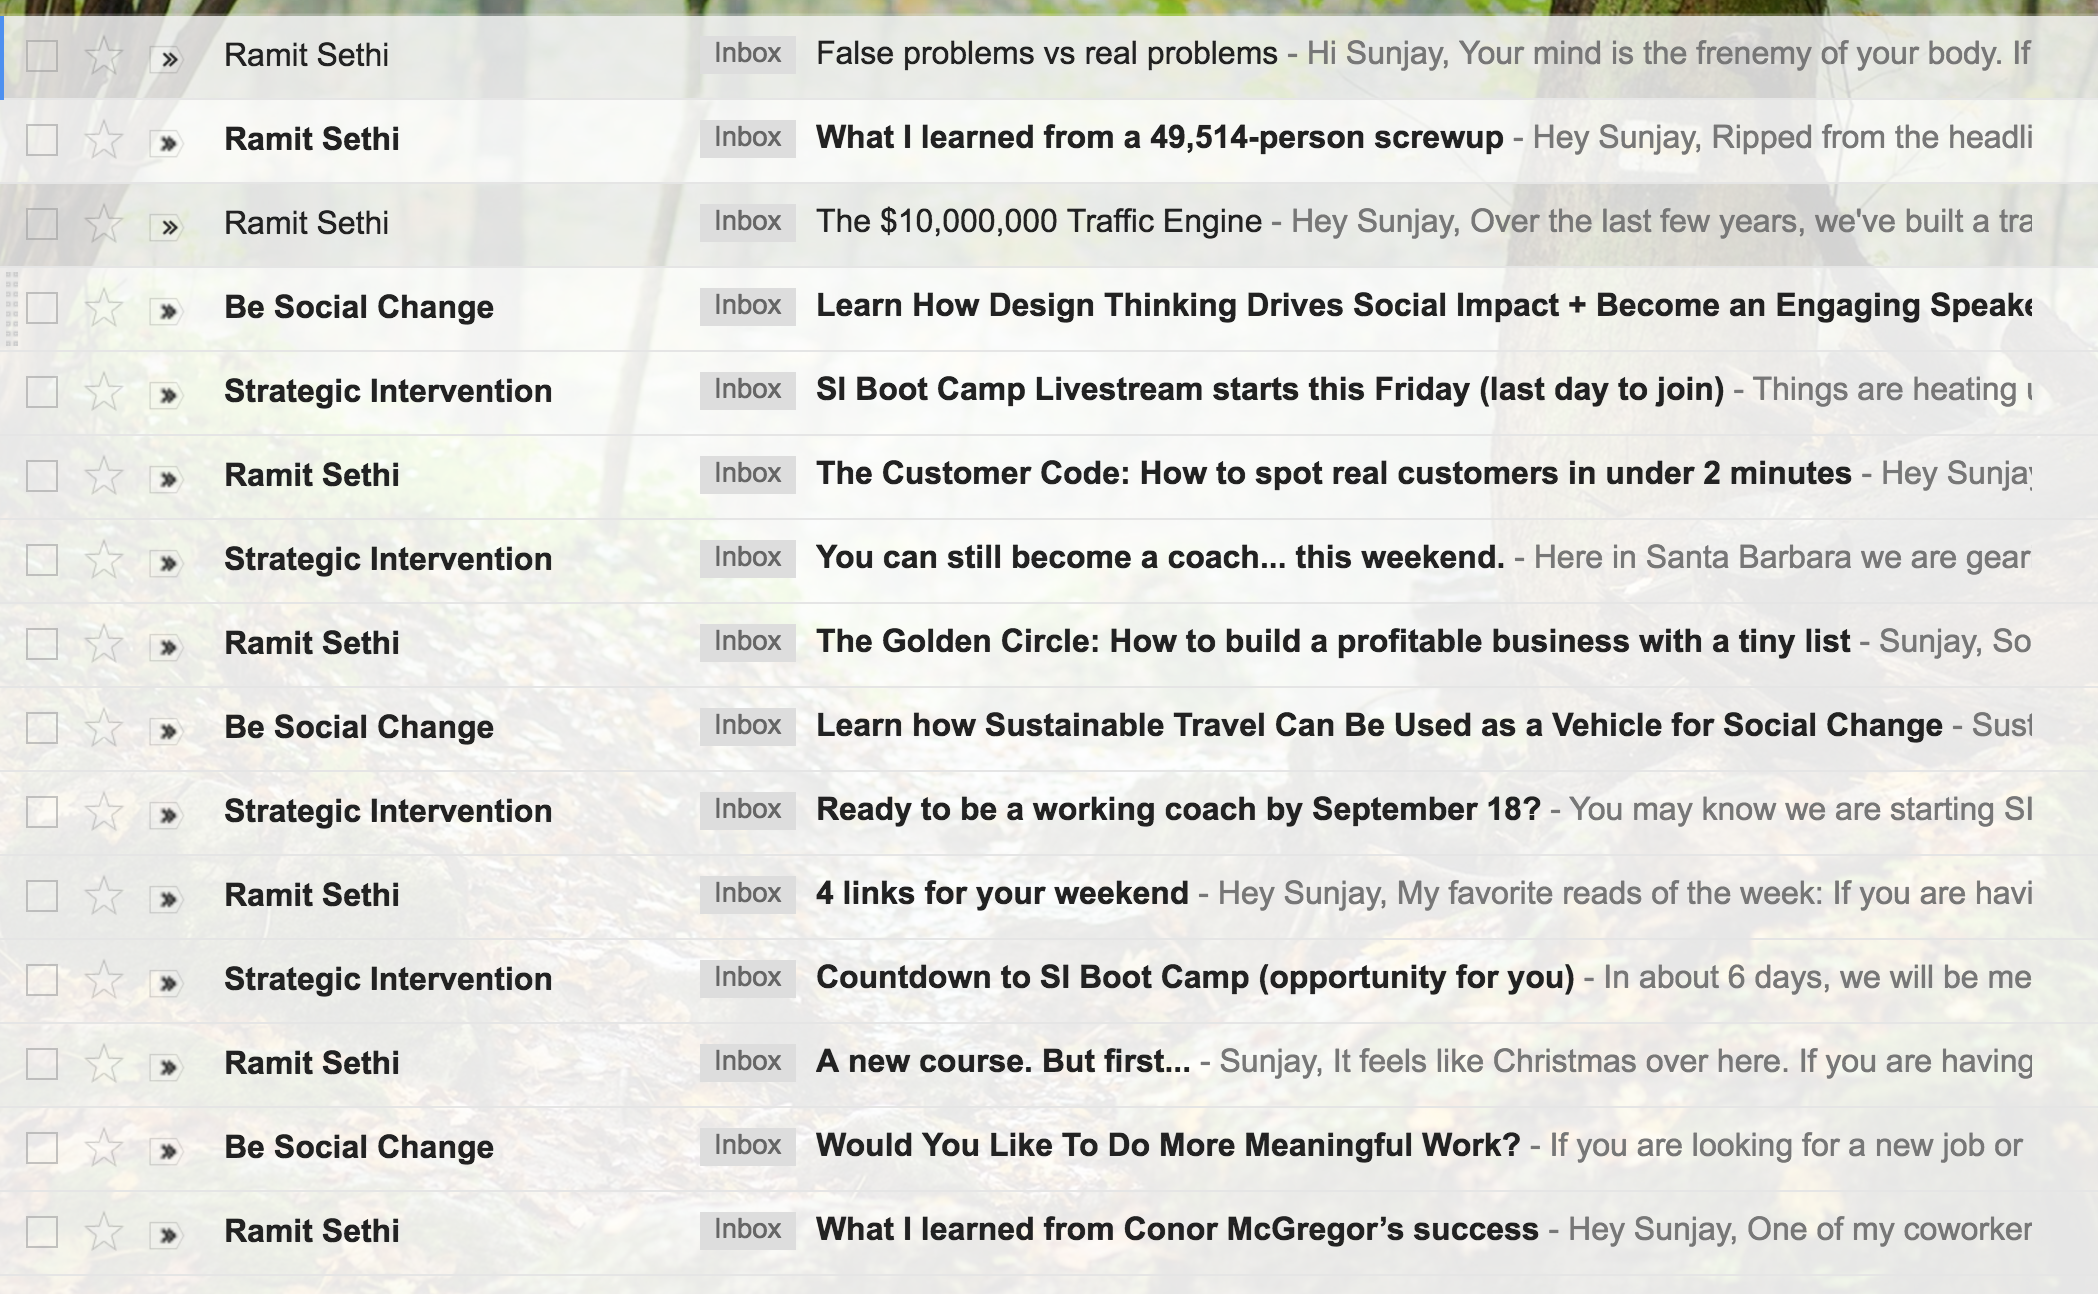
\includegraphics[width=.9\linewidth]{/Users/jay/Dropbox/github/org-html-webslides/assets/img/promise-benefit.png}
\end{center}

\subsection[Headlines]{Headlines\hfill{}\textsc{slide}}
\label{sec:org7770341}
\begin{center}
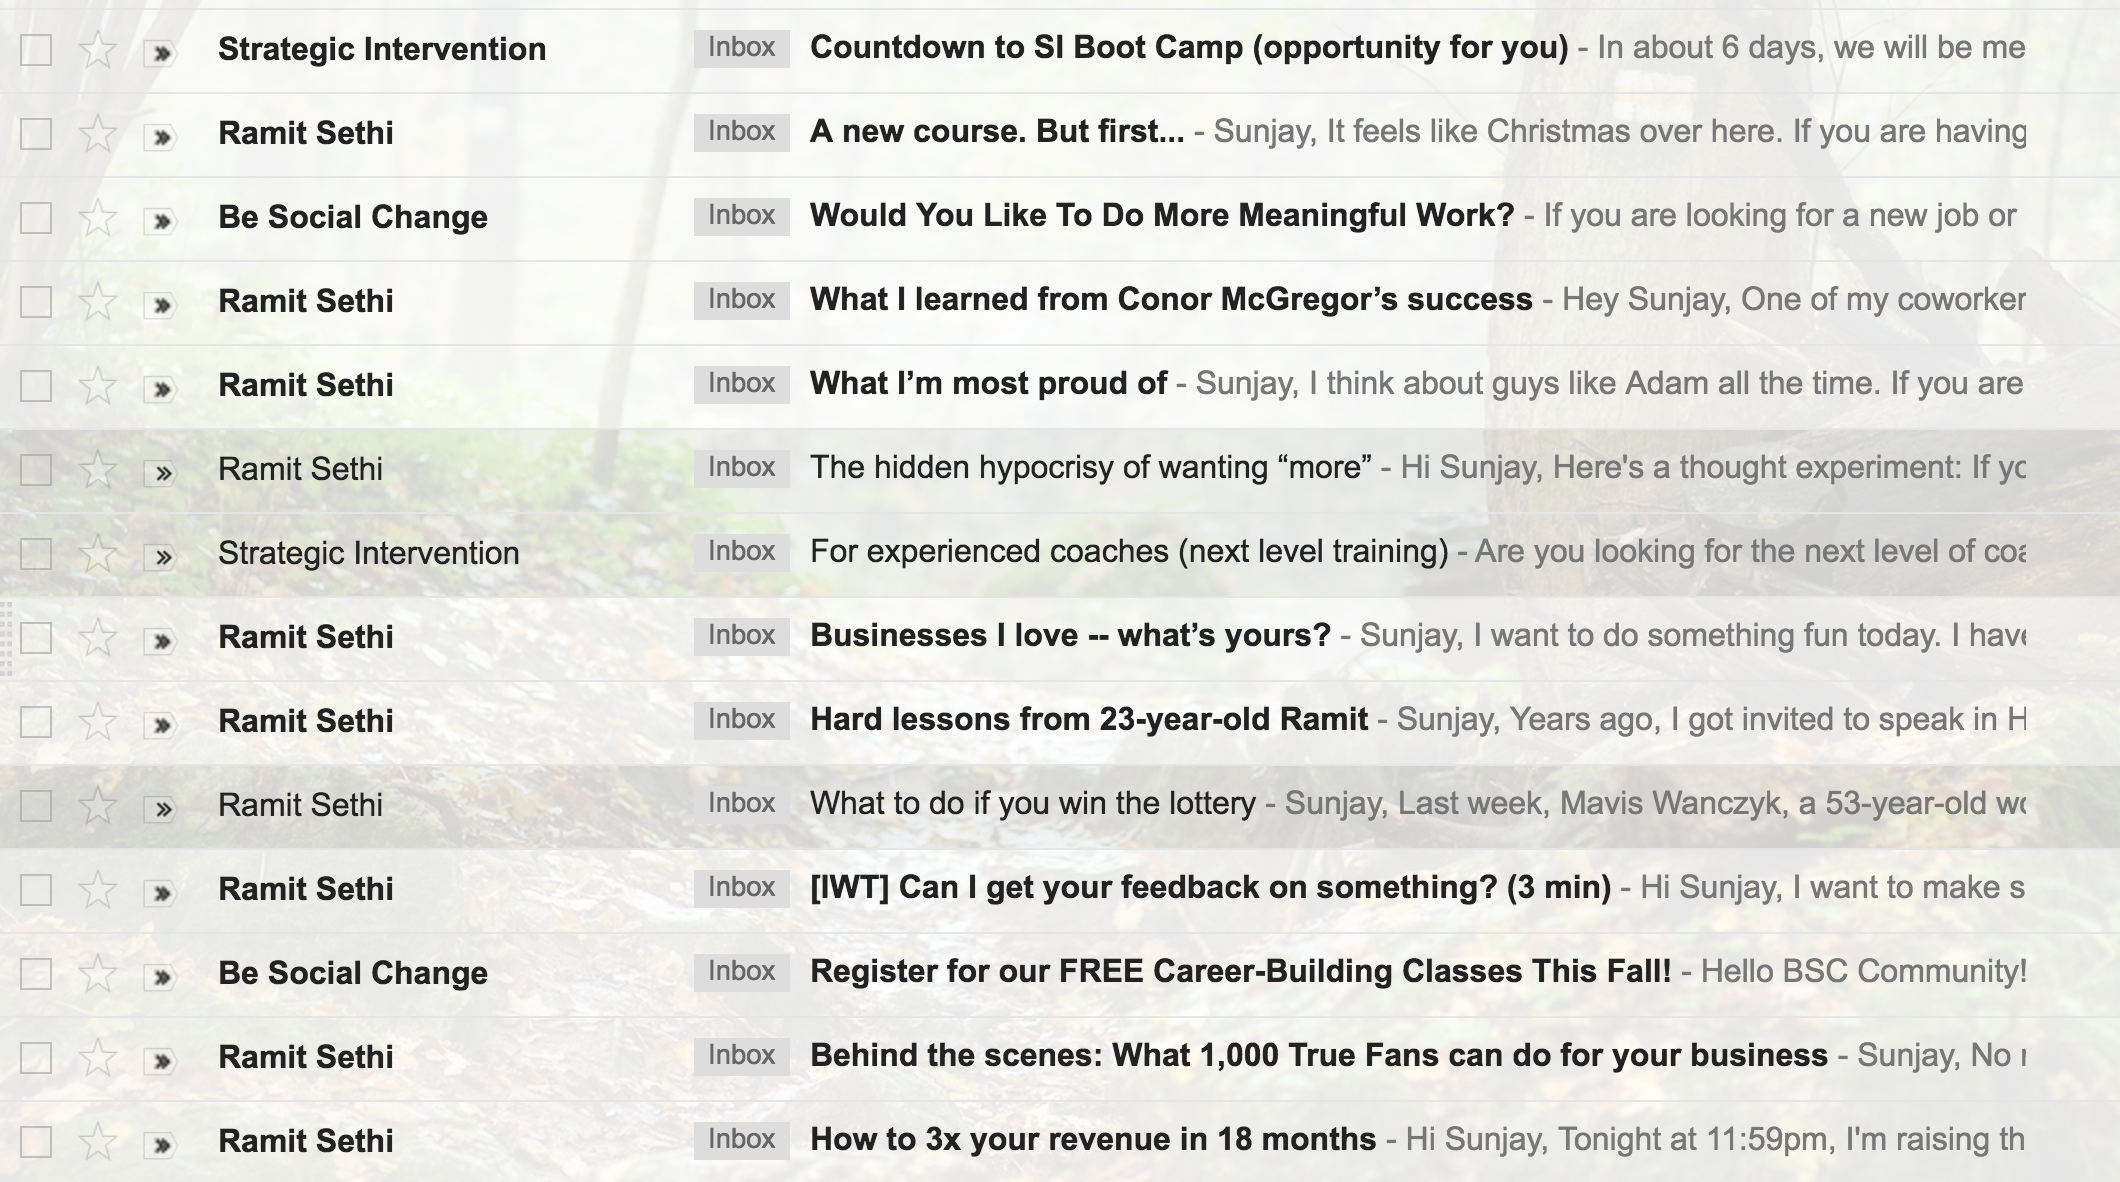
\includegraphics[width=.9\linewidth]{/Users/jay/Dropbox/github/org-html-webslides/assets/img/questions.png}
\end{center}

\subsection[Humor]{Humor\hfill{}\textsc{slide}}
\label{sec:orgb7e988c}
\begin{center}
\includegraphics[width=.9\linewidth]{/Users/jay/Dropbox/storytelling-assets/images/icons/human-icon.png}
\end{center}


\subsection{Headlines}
\label{sec:orgdac1810}
\begin{itemize}
\item curiosity
\item incomplete information (the missing piece)
\item verbs
\item questions
\item benefit / promises
\end{itemize}

\subsection{visual}
\label{sec:org09bb31d}
verbs

\subsection[Curiosity]{Curiosity\hfill{}\textsc{slide:full}}
\label{sec:orgfdefea1}
\begin{center}

\includegraphics[width=.9\linewidth]{/Users/jay/Dropbox/github/org-html-webslides/assets/img/curiosity-icon.jpg}
\end{center}


What are things that create curiosity?

\begin{itemize}
\item unexpected
\item incongruity
\item surprise
\item questions
\end{itemize}

\subsection[The End]{The End\hfill{}\textsc{slide}}
\label{sec:orgd4c54b4}


\subsection[A different approach - longer, outbound email]{A different approach - longer, outbound email\hfill{}\textsc{slide}}
\label{sec:org1d51940}
\begin{quote}
Hi Ellen,

Good to hear from you, and thank you so much for reaching out. Absolutely, I'd be more than happy to talk about how NLI can help you with your D\&I strategy.

As you begin to think about how to address diversity and inclusion at Sanfino, I'll start by saying I think this is a really tricky challenge. Studies show that \href{https://hbr.org/2016/07/why-diversity-programs-fail}{most D\&I programs fail} because they all make the same mistake: they attempt to make individuals less biased.

That approach is doomed to fail because the biases that affect D\&I are unconscious, operating below our awareness and outside our control. Unfortunately, what this means is that a lot of companies pour millions of dollars into programs that ultimately don't increase diversity.

At NLI, we take a different approach. Instead of attempting to make \textbf{individuals} less biased, we focus on taking the bias out of \textbf{decisions}, teaching organizations how to structure processes so as to sidestep the pitfalls of our biased brains.

So far it seems to be working. We've helped improve decision making at 40 companies, including \href{https://neuroleadership.com/portfolio-items/case-study-blackrock-breaking-bias/}{BlackRock} and \href{https://neuroleadership.com/portfolio-items/nli-transforms-intel-culture/}{Intel}, and most of our clients still use our tools at least once a week.

I'd love to set up a time to talk on the phone so I can hear more about your objectives. I'm available for a quick call at the following times:

\begin{itemize}
\item Monday Oct 6, 1:00pm
\item Wednesday Oct 8, 4:00pm
\item Friday Oct 10, 9:00am
\end{itemize}

Do any of those times work for you?

I look forward to connecting!

Best, \\
Jay
\end{quote}


\section{Setup}
\label{sec:org5914d9e}


\subsection[The End]{The End\hfill{}\textsc{slide}}
\label{sec:orge3f8110}

Sometimes it's safest to add an ``empty'' heading at the end of your document to make sure the stylesheets and JavaScript are included.


\subsubsection[Notes]{Notes\hfill{}\textsc{notes}}
\label{sec:org59b411f}

\begin{itemize}
\item Presenter notes for this slide
\item Not displayed as part of the slide
\item Displayed in Presenter Preview window
\item Only one notes section per slide allowed
\end{itemize}

\subsubsection[Notes]{Notes\hfill{}\textsc{Notes}}
\label{sec:org585b5d8}

\textbf{Bad example}
\begin{itemize}
\item irrelevant information
\item information without context
\end{itemize}

\textbf{good example}
\begin{itemize}
\item answers the question directly
\item show you understand the problem
\item show you're listening
\end{itemize}
\end{document}
